
\chapter{Possessive constructions}
\label{bkm:Ref155077914}\section{General background}

The topic of this chapter is possessive noun phrases, that is, noun phrases that involve a possessive modifier, the latter being roughly everything that is functionally equivalent to genitives. Following what is now established terminology, I shall speak of “possessor” and “possessee” for the two entities involved in the possessive relation. It should be noted from the start that possessive constructions may express a diversity of relations that sometimes have very little to do with “ownership”, which has traditionally been seen as their basic meaning. 

When it comes to the expression of possessive relations in noun phrases, Scandinavian languages display a bewildering array of constructions. Quite often, we find a number of competing possibilities within one and the same variety. In this chapter, my main concern will be with lexical possessive NPs – constructions where the possessor is a full NP rather than a pronoun. This includes possessor NPs with different kinds of heads – most notably, the head may be either (i) a proper name or an articleless kin term such as ‘father’, or (ii) a common noun, usually in the definite form. \citet{Delsing2003a} treats these two types under separate headings, which is motivated by the fact that some constructions show up with the first type only. However, as he himself notes, there are no constructions which categorically exclude this type. 

A caveat here about the available material: noun phrases with full NP possessors are less frequent in spoken and informal written language than one would like as a linguist studying this construction, making it difficult to collect enough data to formulate safe generalizations about usage. 

\section{\textit{S-}genitive: old and new}

The traditional device for marking possessive constructions in Indo-European is the genitive case. In older Germanic, like in its sister branches, the genitive also had various other functions – thus, both verbs and prepositions could govern the genitive. This situation is still preserved in some of the modern Germanic languages, such as (Standard) German and Icelandic. In most Germanic varieties, however, the genitive case has either been transformed or has disappeared altogether. Thus, in languages such as Dutch and West Frisian, like in many spoken Scandinavian varieties, we obtain what Koptjevskaja-\citet{Koptjevskaja-Tamm2003 calls “deformed genitives”. In these, what is kept from the traditional genitive case is primarily the suffixal marking, usually a generalized suffix such as\textit{ {}-s}\textstyleLinguisticExample{. }Other common characteristics of deformed genitives are that the possessor phrase is preposed relative to the head noun and that there are restrictions on what kinds of NPs can occur as possessors – in the strictest cases, only proper names and name-like kinship terms. Syntactically, deformed genitives tend to behave more like “determiners” than like “modifiers”, which, among other things, means that they do not co-occur with definite articles. Even in Standard German, where the old genitive is in principle fairly well preserved, there is arguably an alternative “deformed” construction of this kind (e.g. \textstyleLinguisticExample{Peters Buch }‘Peter’s book’\textit{).} If we look at Central Scandinavian, we find a possessive construction which resembles the “deformed genitives” in several ways, but which also differs significantly from it. What is rather curious is that a construction with almost exactly the same properties is found in English – the so-called \textstyleLinguisticExample{s}{}-genitive. The English and Scandinavian constructions share with each other and with the garden-variety deformed genitive at least three properties: (i) the preposed position in the noun phrase; (ii) the generalized \textstyleLinguisticExample{s-}suffix; (iii) the lack of definite marking on the possessee NP or its head noun. They differ from other deformed genitives in not being restricted to proper names and kinship terms and in being possible with basically any noun phrase, regardless of syntactic complexity. The marker\textit{ {}-s} is always on the last element of the noun phrase, which may entail “group genitives” such as Swedish \textstyleLinguisticExample{far mins bok} ‘my father’s book’ or English \textstyleLinguisticExample{Katz and Fodor’s theory}, where the\textit{ {}-s}\textstyleLinguisticExample{ }is not suffixed to the head noun but rather to a postposed modifier or to the last element of a conjoined NP. 

\textit{S}{}-genitives, so characterized, are not found generally in Scandinavian, but are in fact essentially restricted to “Central Scandinavian”, that is, standard Danish and Swedish, with a somewhat reluctant extension to some forms of standard Norwegian and the spoken varieties of southern Scandinavia (south of the \textstyleLinguisticExample{limes norrlandicus}). Even in parts of southern Sweden, however, deviant systems are found. Thus, in central parts of the province of Västergötland, according to the description in \citet{Landtmanson1952}, the ending\textit{ {}-a} is commonly found with proper names and kinship terms. This is also in accordance with the usage in the single Cat Corpus text from that province, the title of which is \textstyleLinguisticExample{Mormora Misse} ‘Granny’s cat’ (likewise, in the same text: \textstyleLinguisticExample{Allfrea kâring} ‘Alfred’s wife’). The ending\textit{ {}-s} is found with a few types of proper names and also with common nouns, “to the extent they can be used in the genitive at all” (\citet[68]{Landtmanson1952}). Genitive forms in\textit{ {}-a} are also found in some Upplandic dialects. In Written Medieval Swedish, Wessén (1968: I:142) notes that the original\textit{ {}-a}\textstyleLinguisticExample{r} ending of \textstyleLinguisticExample{i-} and \textstyleLinguisticExample{u-}stems, often reduced to\textit{ }\textit{{}-}\textit{a},  survived for quite a long time with proper names, “especially in foreign ones”. “In Västergötland and Småland it even still survives: \textstyleLinguisticExample{Davida} ‘David’s’ etc.” The\textit{ {}-a}\textstyleLinguisticExample{r} ending, in non-reduced form, is also found in Orsa (Os): \textstyleLinguisticExample{Alfredar keling} ‘Alfred’s wife’ (but \textstyleLinguisticExample{Momos Måssä} ‘Granny’s cat’, with an \textstyleLinguisticExample{s-}ending).

 More elaborate genitive forms are sometimes found. Thus, in the Cat Corpus text from Träslövsläge (Ha) we find the ending\textit{ {}-s}\textstyleLinguisticExample{a}, as in \textstyleLinguisticExample{Mormosa katt }‘Granny’s cat’ and \textstyleLinguisticExample{Alfredsa käring }‘Alfred’s wife’. The ending\textit{ {}-s}\textstyleLinguisticExample{a} is apparently a combination of the two endings\textit{ {}-s} and\textit{ {}-a}\textstyleLinguisticExample{. }It is also found in Faroese possessives, and in the Alunda vernacular (Up) as described in \citet{Bergman1893}. In the text from Sotenäs in Bohuslän the ending is\textit{ {}-s}\textstyleLinguisticExample{es}, apparently a doubling of\textit{ {}-s}: \textstyleLinguisticExample{Mormorses pissekatt} ‘Granny’s pussy cat’ and \textstyleLinguisticExample{Alfreses kjäreng} ‘Alfred’s wife’ (see \citet{Janzén1936} for a discussion of\textit{ {}-s}\textstyleLinguisticExample{es} forms in Bohuslän vernaculars). Compare also similar examples from Hälsingland with definite forms of the possessee under \sectref{sec:5.3}. 

In the vernaculars of the Peripheral Swedish area, like in most of Norway, the \textstyleLinguisticExample{s}{}-genitive, at least in its canonical form as described above, is generally absent or weakly represented in a way that suggests late influence from acrolectal varieties. \citet[41]{Delsing2003a} says that the \textstyleLinguisticExample{s}{}-genitive is totally absent in the “old dative vernaculars” of Norrbotten and coastal northern Västerbotten, as well as in Jämtland and Härjedalen as well as in the Dalecarlian area. In the rest of northern and middle Norrland there are only few attestations, he says, and they seem to be a “young phenomenon”. On the whole, the weak support for the \textstyleLinguisticExample{s}{}-genitive in the vernaculars of peninsular Scandinavia, with the exception of the Southern Swedish/East Danish dialect area, is striking. In fact, it appears to me that the development of the \textstyleLinguisticExample{s}{}-genitive, as described e.g. by \citet{Norde1997},\footnote{ Norde describes the development of the \textit{s}{}-genitive as an essentially internal phenomenon in Swedish and does not treat deviant developments in vernaculars or draw parallels to Danish.} may be essentially restricted to Danish, Scanian and prestige or standard varieties of Swedish, and possibly some parts of Götaland. 

\section{Definite in \textit{s-}genitives}
\label{sec:5.3}

A construction which is fairly analogous to the standard \textstyleLinguisticExample{s}{}-genitive – differing from it primarily in that the head noun takes the definite form – is found in a relatively large part of the Peripheral Swedish area on both sides of the Baltic (\citet[27]{Delsing2003a}).

In Mainland Sweden, the strongest area seems to be Hälsingland. In the Cat Corpus, it is found in all three texts from this province, although alternating with the regular \textit{s}{}-genitive construction. Thus, for ‘Alfred’s wife’ we find \textstyleLinguisticExample{Alfreds käringa} from Järvsö (Hä) and \textstyleLinguisticExample{Alfreses tjeringa} from Färila (Hä), with a doubled ending\textit{ {}-ses}, and \textstyleLinguisticExample{frua Alfreds}, with the order possessee-possessor, from Forsa (Hä). Further north, it is less common, but does occur.  Bergholm et al. found cases such as \textstyleLinguisticExample{Pers bole }‘Per.{\gen} table.{\def}’ and \textstyleLinguisticExample{mine brorn} ‘my brother.{\def}’ in Burträsk (NVb). \citet[27]{Delsing2003a} enumerates quite a few examples from the literature and from written texts, covering all the coastal provinces in Norrland except Norrbotten, and also the Laplandic parts of the Westrobothnian area. 

The construction is also found in Gotland, as in the Cat Corpus examples \textstyleLinguisticExample{Mormors sänge} ‘Granny’s bed’ from Fårö (Go) and \textstyleLinguisticExample{Mårmårs sänggi }‘Granny’s bed’ from Lau (Go). In Gotland, definite forms can also be used with pronominal possessors, as in \REF{247}.

\ea\label{}
\langinfo{\label{bkm:Ref155247297}Lau (Go)}{}{}\\
\gll De  jär  \textbf{min} \textbf{kattn.}\\
it  be.{\prs}  \textbf{my} \textbf{cat.{\def}}\\
\glt  ‘It is my cat.’ (Cat Corpus)
\z

The construction seems to be general in the whole Trans-Baltic area. In most cases, the possessor takes the affix\textit{ {}-s}, but in Ostrobothnian\textit{ {}-as }is also quite common – I shall return to this in \sectref{sec:5.4.2}. In Ostrobothnian, \citet{ErikssonEtAl1999} also found considerable variation between definite and indefinite possessees – roughly 50 per cent of each. 

From older times, \citet[523]{Hesselman1908} quotes examples from the 17\textsuperscript{th} century lexicographer Ericus Schroderus such as

\ea\label{}
\langinfo{Upplandic (17\textsuperscript{th} century)}{}{}\\
\gll Lijffzens  Träet\\
life.{\gen}.{\def}  tree.{\def}\\
\glt  ‘the tree of life’
\z

%\begin{styleTextkrper}
and from Bureus, another 17\textsuperscript{th} century writer:

%\end{styleTextkrper}

\ea\label{}
\langinfo{Upplandic (17\textsuperscript{th} century)}{}{}\\
\gll hos  Anders  Burmans  i  Rödbäck  systren\\
at  Anders  Burman.{\gen}  in  Rödbäck  sister.{\def}\\
\glt ‘at the sister of Anders Burman in Rödbäck’
\z

and says “in the same way as modern Upplandic: \textit{Geijers dalen }[Geijer’s Valley], \textit{bokhandlarens pojken} ‘the bookseller’s boy’ etc.” This is the only place in the literature known to me where definites with \textit{s}{}-genitives are said to be found in Upplandic. (The first example is clearly a compound in the modern language, spelled \textit{Geijersdalen}.)

As for the alternative construction with the possessee-possessor word order, found in the example from Forsa (Hä) above, Delsing quotes a number of examples, some of them, as he says, “from unexpected places” such as Värmland and Västergötland. The word order possessee-possessor was normal in Old Nordic and is still used in Icelandic (although without definite marking on the possessee). It is thus possible that it is an archaism at least in some places – although hardly for the Laplandic vernaculars mentioned by Delsing.

\section{Constructions with the dative}
\label{sec:5.4}\subsection{The plain dative possessive}\label{sec:5.4.1}

In many Peripheral Swedish vernaculars, a common possessive construction involves a dative-marked possessor. In most cases, the word order is possessed-possessor, but preposed possessors also occur. The possessee NP is normally morphologically definite only when it precedes the possessor. I shall call this construction \textbf{the plain dative possessive}. The following two phrases exemplify the postposed and preposed variants of this construction:

\renewcommand{\eachwordone}{\scshape}
\renewcommand{\eachwordtwo}{\itshape}

\ea\label{}
	\langinfo{\textit{Skelletmål} (NVb)}{}{}\\
	\glll \textbf{\textsc{possessee}} \textbf{\textsc{possessor}} \\
	skoN  paitjåm  \\
	shoe.{\sg}.{\def}  boy.{\dat}.{\sg}.{\def}  \\
	\glt ‘the boy’s shoe’ (\citet[22]{Marklund1976})
\z

\ea\label{}
	\langinfo{\label{bkm:Ref95906318}Nederkalix (Kx)}{}{}\\
	\glll \textbf{\textsc{possessor}} \textbf{\textsc{possessee}} \\
	Mårmorn  kjaatt\\
	Granny.{\def}.{\dat}  cat\\
\glt ‘Granny’s cat’ (Cat Corpus, title of translation)
\z

Even in those vernaculars where the dative is preserved, cases of zero-marking are common. Thus, many examples of this construction look like plain juxtaposition of two NPs:

\ea\label{}
	\langinfo{\label{bkm:Ref134419452}Älvdalen (Os)}{}{}\\
	\glll \textbf{\textsc{possessee}} \textbf{\textsc{possessor}} \\
	kalln  Smis-Margit \\
	man.{\def}.{\sg}  Smis-Margit\\
\glt ‘Smis-Margit’s husband’ (\citet[97]{Levander1909})
\z

In examples such as \REF{252}, the possessor NPs can be regarded as being in the dative – the lack of overt marking is in accordance with the grammar of the vernacular. However, there are also examples where an expected overt marking is lacking. For instance, in the Cat Corpus, we find in addition to the dative-marked \REF{251} an example such as \REF{253}, with the nominative \textstyleLinguisticExample{mårmora} ‘Granny’: 

\renewcommand{\eachwordone}{\itshape}


\ea\label{}
\langinfo{\label{bkm:Ref110681866}Nederkalix (Kx)}{}{}\\
\gll Hån  Murre  sprant  åopp\\
{\pda}.{\m}  Murre  jump.{\pst}  up\\
\gll å  laar  ’se  opa  \textbf{måan} \textbf{mårmora.}\\
and  lay  {\refl}  on  \textbf{belly.{\def}} \textbf{Granny.{\def}}\\
\glt ‘Murre jumped up and lay down on Granny’s belly.’ (Cat Corpus)
\z

\citet[161--163]{Källskog1992} treats the possessive dative in the Överkalix vernacular (Kx) in some detail and says that it is “perhaps the most common way of expressing the genitive concept”.\footnote{ “Det kanske vanligaste sättet att uttrycka genitivbegreppet i överkalixmålet är att använda en omskrivning med dativ.” It is not clear why Källskog uses the term \textit{omskrivning} ‘periphrasis’ here – it would seem that the dative construction is not more periphrastic than the \textit{s-}genitive.} She enumerates five possibilities:

\renewcommand{\eachwordone}{\scshape}

\begin{enumerate}
\item[1] Definite possessee + definite possessor in the dative
\end{enumerate}

%\end{listLFOxvileveli}

\ea\label{}
\langinfo{Överkalix (Kx)}{}{}\\
\ea {
\glll \textbf{\textsc{possessee}}  \textbf{\textsc{possessor}}\\
stjella  fa:ren  iert\\
bell  sheep.{\dat}  your.{\n}\\
\glt ‘the bell of your sheep’
}

\ex {
\glll \textbf{\textsc{possessee}}  \textbf{\textsc{possessor}}\\
möylhn  stäjntn  hina\\
ball.{\def}  girl.{\dat}  this.{\f}\\
\glt ‘this girl’s ball’
}
\z 
\z 

\begin{enumerate}
\item[2] Definite possessor in the dative + indefinite possessee
\end{enumerate} 

\ea\label{}
\langinfo{Överkalix (Kx)}{}{}\\
\ea { 
\glll \textbf{\textsc{possessor}}  \textbf{\textsc{possessee}}\\
	färssfe:ro  djey$\lambda $\\
	paternal\_grandfather.{\dat}  field\\
\glt ‘Grandfather’s field’
}

\ex {
\glll \textbf{\textsc{possessor}} \textbf{\textsc{possessee}}\\
kwäjen  ka$\lambda $v\\
heifer.{\dat}  calf\\
\glt ‘The heifer’s calf has black and red spots.’
}
\z 
\z

\begin{enumerate} 
\item[3] Indefinite possessee + indefinite possessor in the dative
\end{enumerate} 

\ea 
\langinfo{Överkalix (Kx)}{}{}\\
\glll \textbf{\textsc{possessee}} \textbf{\textsc{possessor}}\\
in  hesst  ino  åokonna  kär\\
{\indf}  horse  {\indf}.{\dat}.{\m}  unknown  man\\
\glt  ‘an unknown man’s horse’
\z

\begin{enumerate}
\item[4] Indefinite possessee + definite possessor in the dative
\end{enumerate} 

%\end{listLFOxvileveli}

\ea\label{}
\langinfo{Överkalix (Kx)}{}{}\\
\glll \textbf{\textsc{possessee}} \textbf{\textsc{possessor}}\\
in  så:n  sistern\\
{\indf}  son  sister.{\def}.{\dat}\\
\glt ‘a son of my sister’
\z

%\begin{styleListeii}
\begin{enumerate}
\item[5] Possessor without case-marking + indefinite possessor
\end{enumerate}

%\end{listLFOxvileveli}

\ea\label{}
\langinfo{Överkalix (Kx)}{}{}\\
\glll \textbf{\textsc{possessor}} \textbf{\textsc{possessee}}\\
mäjn  ba:n  laigseker\\
my  child.{\pl}  toy.{\pl}\\
\glt ‘my children’s toys’
\z

The first, third and fourth possibilities clearly represent the postposed variant of the plain dative possessive, and the second possibility the preposed variant. In the fifth case, the dative has been replaced by the nominative.  

\citet{Rutberg1924}, in her description of \textit{Nederkalixmål}, presents paradigms where the genitive and the dative are identical throughout. Both \citet[161]{Källskog1992} and \citet[42]{Delsing2003a} take this as an indication that dative-marked possessors are possible. Indeed, the Cat Corpus text from Nederkalix contains at least three clear examples – \REF{251} above and also the following:

\renewcommand{\eachwordone}{\itshape}


\ea\label{}
\langinfo{Nederkalix (Kx)}{}{}\\
\gll Utimila  var  ‘e  för  varmt  baki  \textbf{röyggen} \textbf{mårmorn.}\\
sometimes  be.{\pst}  it  too  hot  behind  \textbf{back.{\def}} \textbf{Granny.{\def}.{\dat}}\\
\glt ‘[The cat thought:] Sometimes it was too hot behind Granny’s back.’ (Cat Corpus)
\z

\ea\label{}
\langinfo{Nederkalix (Kx)}{}{}\\
\gll mårmorn  vé\\
Granny.{\def}.{\dat}  firewood\\
\glt ‘Granny’s firewood’  (Cat Corpus)
\z

For \textit{Lulemål}, \citet{Nordström1925} says that the genitive, like the dative, takes the ending\textit{ {}-o}. He gives the example \textstyleLinguisticExample{färo mööss} ‘father’s cap’. In the Cat Corpus, there are examples from \textit{Lulemål} such as \textstyleLinguisticExample{Mormoro lillveg} ‘Granny’s little road’.  \citet[163]{Källskog1992} quotes two proverbs from transcriptions done by E. Brännström, interpreting the \textstyleLinguisticExample{o}{}-ending as a dative marker: 

\ea\label{}
\langinfo{Nederluleå (Ll)}{}{}\\
\ea {
\gll Fisk  o  bröd  jer  \textbf{bånndo} \textbf{fööd.}\\
fish  and  bread  be.{\prs}  \textbf{farmer.{\def}.{\dat}} \textbf{food}\\
\glt ‘Fish and bread are the farmer’s food.’
}

\ex {
\gll He  jer  ållt  \textbf{bånndo} \textbf{arrbäjt.}\\
it  be.{\prs}  clearly  \textbf{farmer.{\def}.{\dat}} \textbf{work}\\
\glt ‘It is clearly the farmer’s work.’
}
\z 
\z

She also mentions an expression \textstyleLinguisticExample{måora pappen} ‘father’s mother’, said to be obsolete, by a speaker born in 1898.

From Böle in Råneå parish (Ll), \citet[113]{Wikberg2004} quotes examples such as \textstyleLinguisticExample{gråsshändlaro daoter} ‘the wholesale trader’s daughter’ and \textstyleLinguisticExample{maoro klening} ‘Mother’s dress’ together with juxtapositional cases such as \textstyleLinguisticExample{pappen råck} ‘Father’s coat’ and \textstyleLinguisticExample{mammen tjaol} ‘Mother’s skirt’.

For \textit{Pitemål}, \citet[11]{Brännström1993} mentions the postposed construction as “obsolete” (ålderdomligt) and gives the example \textstyleLinguisticExample{påtjen fàrom} ‘Father’s boy’. 

Moving south to northern Westrobothnian, we have already seen one case of the possessive dative from \textit{Skelletmål} as described by \citet[22]{Marklund1976}, who also gives the following examples: \textstyleLinguisticExample{löNa pi{\textasciigrave}gen} ‘the maid’s pay’, \textstyleLinguisticExample{rissla græ{\textasciigrave}nnåm} ‘the neighbour’s sleigh’, \textstyleLinguisticExample{kæppa n’Greta} ‘Greta’s coat’, \textstyleLinguisticExample{löngNeN n’Lova} ‘Lova’s lies’, \textstyleLinguisticExample{hästn åm Jâni }‘Johan’s horse’. 

In his discussion of the Lövånger (NVb) vernacular, \citet[208]{Holm1942} says that “there are a great number of other possibilities” than the \textit{s}{}-genitive of the standard language (which he says is not possible in the vernacular), and gives as an example juxtaposition with the order possessee–possessor, as in \textstyleLinguisticExample{rävapälsen pastor Holm} ‘the Reverend Holm’s fox fur coat’. 

\citet[125]{Larsson1929} reports postposed possessives both with and without dative marking from Westrobothnian, without indicating any specific geographical locations. About the juxtapositional construction, he says that it is “very common” and gives examples such as the following:

\begin{table}
\begin{tabular}{ll}
\lsptoprule Westrobothnian & English \\
\midrule 
\textit{skon pötjen} & ‘the boy’s shoes’\\ 
\textit{nesdutjen stinta} & ‘the girl’s handkerchief’\\ 
\textit{lönja piga} & ‘the maid’s pay’\\ 
\textit{tjettn fara} & ‘the sheep’s pen’\\ 
\textit{legden Jonson} & ‘Jonsson’s former fields’\\ 
\textit{bökjsen n Nikkje} & ‘Nicke’s trousers’\\ 
\textit{strompen a Greta} & ‘Greta’s stockings’\\
\lspbottomrule
\end{tabular}
\caption{Some nice caption.}
\label{tab:5.1}
\end{table} 

%\end{styleBlockQuote}

For the last two examples, he gives the alternatives \textstyleLinguisticExample{bökjsen hanjs Nikkje} and \textstyleLinguisticExample{strompen hanasj Greta}, both of which should more properly be treated as \textit{h}{}-genitives (see \sectref{sec:5.5}).

For the dative-marked construction, he gives the following examples: \textstyleLinguisticExample{boka prestum} ‘the clergyman’s book’, \textstyleLinguisticExample{lönja pigen} ‘the maid’s pay’,\textstyleLinguisticExample{ löngnen n kesa} ‘Kajsa’s lies’. 

With the reservation that Larsson does not specify the location of his examples, it appears that no attestations of the dative construction are found in southern Westrobothnian, which is perhaps not so astonishing, given that the dative has more or less disappeared there. In order to find further examples of the plain dative construction, we have to move about 700 kilometers south to the Ovansiljan area, where \citet[97]{Levander1909} gives this construction as the normal way of expressing nominal possession in Elfdalian:\footnote{ “Genitivbegreppet uttrycks vanligen genom postponerad dativ”}

\ea\label{}
\langinfo{Älvdalen (Os)}{}{}\\
\gll fjosbuðe;  sturmasum\\
stable-shed.{\def}  Stormas.{\def}-{\pl}\\
\glt ‘the shed of the Stormas people’
\z

As a modern example, we may cite the following:

\ea\label{}
\langinfo{Älvdalen (Os)}{}{}\\
\gll Ulov  add  taið  \textbf{pennskrineð} \textbf{kullun.}\\
Ulov  have.PRET  take.{\sup}  \textbf{pen\_box.{\def}} \textbf{girl:{\dat}.{\sg}.{\def}}\\
\glt ‘Ulov had taken the girl’s pen case.’ (\citet[120]{Åkerberg2012}))
\z

According to \citet[112]{Levander1928}, the plain dative possessive construction is (or was) found in many places in the Dalecarlian area. Outside Älvdalen, he quotes the following examples:

\ea\label{}
\langinfo{Boda (Ns)}{}{}\\
\gll sk\k{u}ônna;  Ierrka\\
shoe.{\pl}  Erik.{\dat}\\
\glt ‘Erik’s shoes’
\z

\ea\label{}
\langinfo{Sollerön (Os)}{}{}\\
\gll g\={ä}rdi  S\={å}rim\\
work.{\pl}  Zorn\\
\glt ‘[the painter Anders] Zorn’s works’ 
\z

\ea\label{}
\langinfo{Transtrand (Vd)}{}{}\\
\gll hätta  dränndjan\\
cap.{\def}  farm-hand.{\dat}\\
\glt ‘the farm-hand’s cap’
\z

For Sollerön, \citet[357]{AnderssonEtAl1999} mention the plain dative possessive as “a nice old locution”,\footnote{ “en gammal och fin ordvändning”} with examples such as the following:

\ea\label{}
\langinfo{Sollerön (Os)}{}{}\\
\gll katto  Margit\\
cat.{\def}  Margit\\
\glt ‘Margit’s cat’
\z

\ea\label{}
\langinfo{Sollerön (Os)}{}{}\\
\gll biln  prässtim\\
car.{\def}  priest.{\def}.{\dat}\\
\glt “the priest’s car”
\z

%\begin{styleTextkrper}
In the Cat Corpus, we find the following examples without overt case-marking:

\ea 
\ea 
\langinfo{Mora}\\
\gl \textit{sendjen Mårmår}\\
\glt ‘Granny’s bed’

\ex 
\langinfo{Mora}\\
\gl \textit{kelindje Alfred}\\
\glt ‘Alfred’s wife’

\ex 
\langinfo{Sollerön}\\
\gl \textit{kelindji Alfred}\\
\glt ‘Alfred’s wife’

\z 
\z

%\end{styleListeiii}

%\end{styleListeiii}

From these data, it appears that the plain dative construction is or has been possible over the whole dative-marking part of the Dalecarlian area. 

Summing up the geographical distribution, we find two areas where dative marking of possessors is employed: Norrbotten and northern Västerbotten, and the Dalecarlian area. A possible difference is that the examples from the northern area tend to involve common nouns whereas proper names also show up fairly frequently in the Dalecarlian examples. 

It may seem a little unexpected to find the dative as a marker of adnominal possession, but there is a relatively plausible diachronic source for it, namely what has been called “external possession” or “possessor raising constructions”. This is a very widespread but by no means universal type of construction in which the possessor of a referent of a noun phrase in a sentence is expressed by a separate noun phrase, marked by an oblique case or a preposition. (English is an example of a language that has no external possessor construction, where adnominal possessors have to be used instead.) The prototypical cases of external possessor constructions involve relational nouns, above all body-part nouns (which are sometimes incorporated into the verb).

In many Indo-European languages, the possessor NP is dative-marked, as in \REF{271}(a), which is more or less synonymous to \REF{271}(b), where the possessor is expressed by an adnominal genitive:

\ea\label{}
\langinfo{\label{bkm:Ref95294441}German}{}{}\\
\ea 
\gll Peter  wusch  \textbf{seinem} \textbf{Sohn} \textbf{die} \textbf{Füße.}\\
Paul  wash.{\pst}  \textbf{his.{\dat}.{\m}.{\sg}} \textbf{son} \textbf{{\def}.{\nom}.{\pl}} \textbf{foot.{\nom}.{\pl}}\\
\ex 
\gll Peter  wusch  \textbf{die} \textbf{Füße} \textbf{seines} \textbf{Sohns.}\\
Paul  wash.{\pst}  \textbf{{\def}.{\nom}.{\pl}} \textbf{foot.{\nom}.{\pl}} \textbf{his.{\dat}.{\m}.{\sg}} \textbf{son}\\
\glt ‘Paul washed his son’s feet.’
\z
\z 

In the older stages of Scandinavian, dative-marked external possessors were also possible. The following example is quoted from the Västgöta provincial law (\citet[15]{Wessén1956}, \citet[212]{Norde1997}): 

\ea\label{}
\langinfo{Early Written Medieval Swedish}{}{}\\
\gll Skiær  tungu  ör  \textbf{höfþi} \textbf{manni…}\\
cut.{\prs}  tongue.{\acc}  out\_of  \textbf{head.{\dat}} \textbf{man.{\dat}}\\
\glt ‘If one cuts the tongue out of a man’s head…’ [S2]
\z

In many Scandinavian varieties, the dative-marked external possessor construction disappeared together with the dative case in general. As a replacement, a periphrastic construction, where the external possessor phrase is marked by the preposition \textstyleLinguisticExample{på} ‘on’, is used in Central Scandinavian including many vernaculars, as in the following example from the Cat Corpus: 

\ea\label{}
\langinfo{Grytnäs (Be) }{}{}\\
\gll Sen  huppa  han  åpp  i  \textbf{knäna} \textbf{på} \textbf{na.}\\
then  jump.{\pst}  he  up  in  \textbf{knee.{\def}.{\pl}} \textbf{on} \textbf{she.{\obl}}\\
\glt ‘Then he jumped onto her lap.’ (Cat Corpus)
\z

As we shall see later, however, in the Peripheral Swedish area, it is more common for another preposition – a cognate of Swedish \textstyleLinguisticExample{åt} and English \textstyleLinguisticExample{at} – to be used in this way.

There are a few examples from early Scandinavian which seem more like adnominal possessors. Thus:

\ea\label{}
	\ea 
		\langinfo{Runic Swedish}{}{}\\
		\gll stuþ  trikila  i  \textbf{stafn} \textbf{skibi}\\
		stand.{\pst}  manly  in  \textbf{stem.{\dat}} \textbf{ship.{\dat}}\\
		\glt ‘He stood manly at the stem of the ship.’ [S35]
	\ex 
		\langinfo{Early Written Medieval Swedish}{}{}\\
		\gll Dræpær  maþer  man, varþær  han  siþen  dræpin  a  \textbf{fotum} \textbf{hanum}\\
		kill.{\prs}  man.{\nom}  man.{\acc} become.{\prs}  he  then  kill.PP  at  \textbf{foot.{\dat}.{\pl}} \textbf{he.{\dat}}\\
		\glt ‘If a man kills a man, and is then killed at his [that man’s] feet.’ [S2]
	\z 
\z

(\citet[15]{Wessén1956}, \citet[211]{Norde1997})

\citet[212]{Norde1997} cites \textstyleLinguisticExample{hanum }in (\ref{274}b) as a clear example of an adnominal possessor. Her criterion is the role of the referent of the dative phrase: “the dead man at whose feet the man who murdered him is killed himself, can hardly be seen as beneficiary of this killing; in this example the dative \textstyleLinguisticExample{hanum} strictly belongs to \textstyleLinguisticExample{fotum}, not to the whole clause”. I do not find this argument wholly convincing, but given their borderline character, examples like (b) could act as a basis for the reinterpretation of external possessor NPs as adnominal possessors. There is little evidence that the process really got off the ground in Written Medieval Swedish.

For Medieval Norwegian, \citet{Larsen1895} claims that the dative tended to be confused with the genitive (which was at the time disappearing) and quotes examples such as \textstyleLinguisticExample{Kiæxstadom vældi} ‘the property of the Kekstad manor’. It is difficult to say how common this phenomenon was, and standard histories of Norwegian such as \citet{SaltveitEtAl1971} do not mention it. To me, it looks more like occasional confusion than a systematic usage – the examples cited by Larsen often seem to have occurred in contexts which would tend to induce the dative (such as following a preposition governing the dative). In any case, there seem to be no traces of the plain possessive dative in Modern Norwegian varieties. On the other hand, it is far from excluded that confusion of this kind may have contributed to the rise of the dative possessive constructions also in Swedish vernaculars. (Some of Larsen’s examples look more like the complex dative possessive, see below.)

\begin{figure}[h]
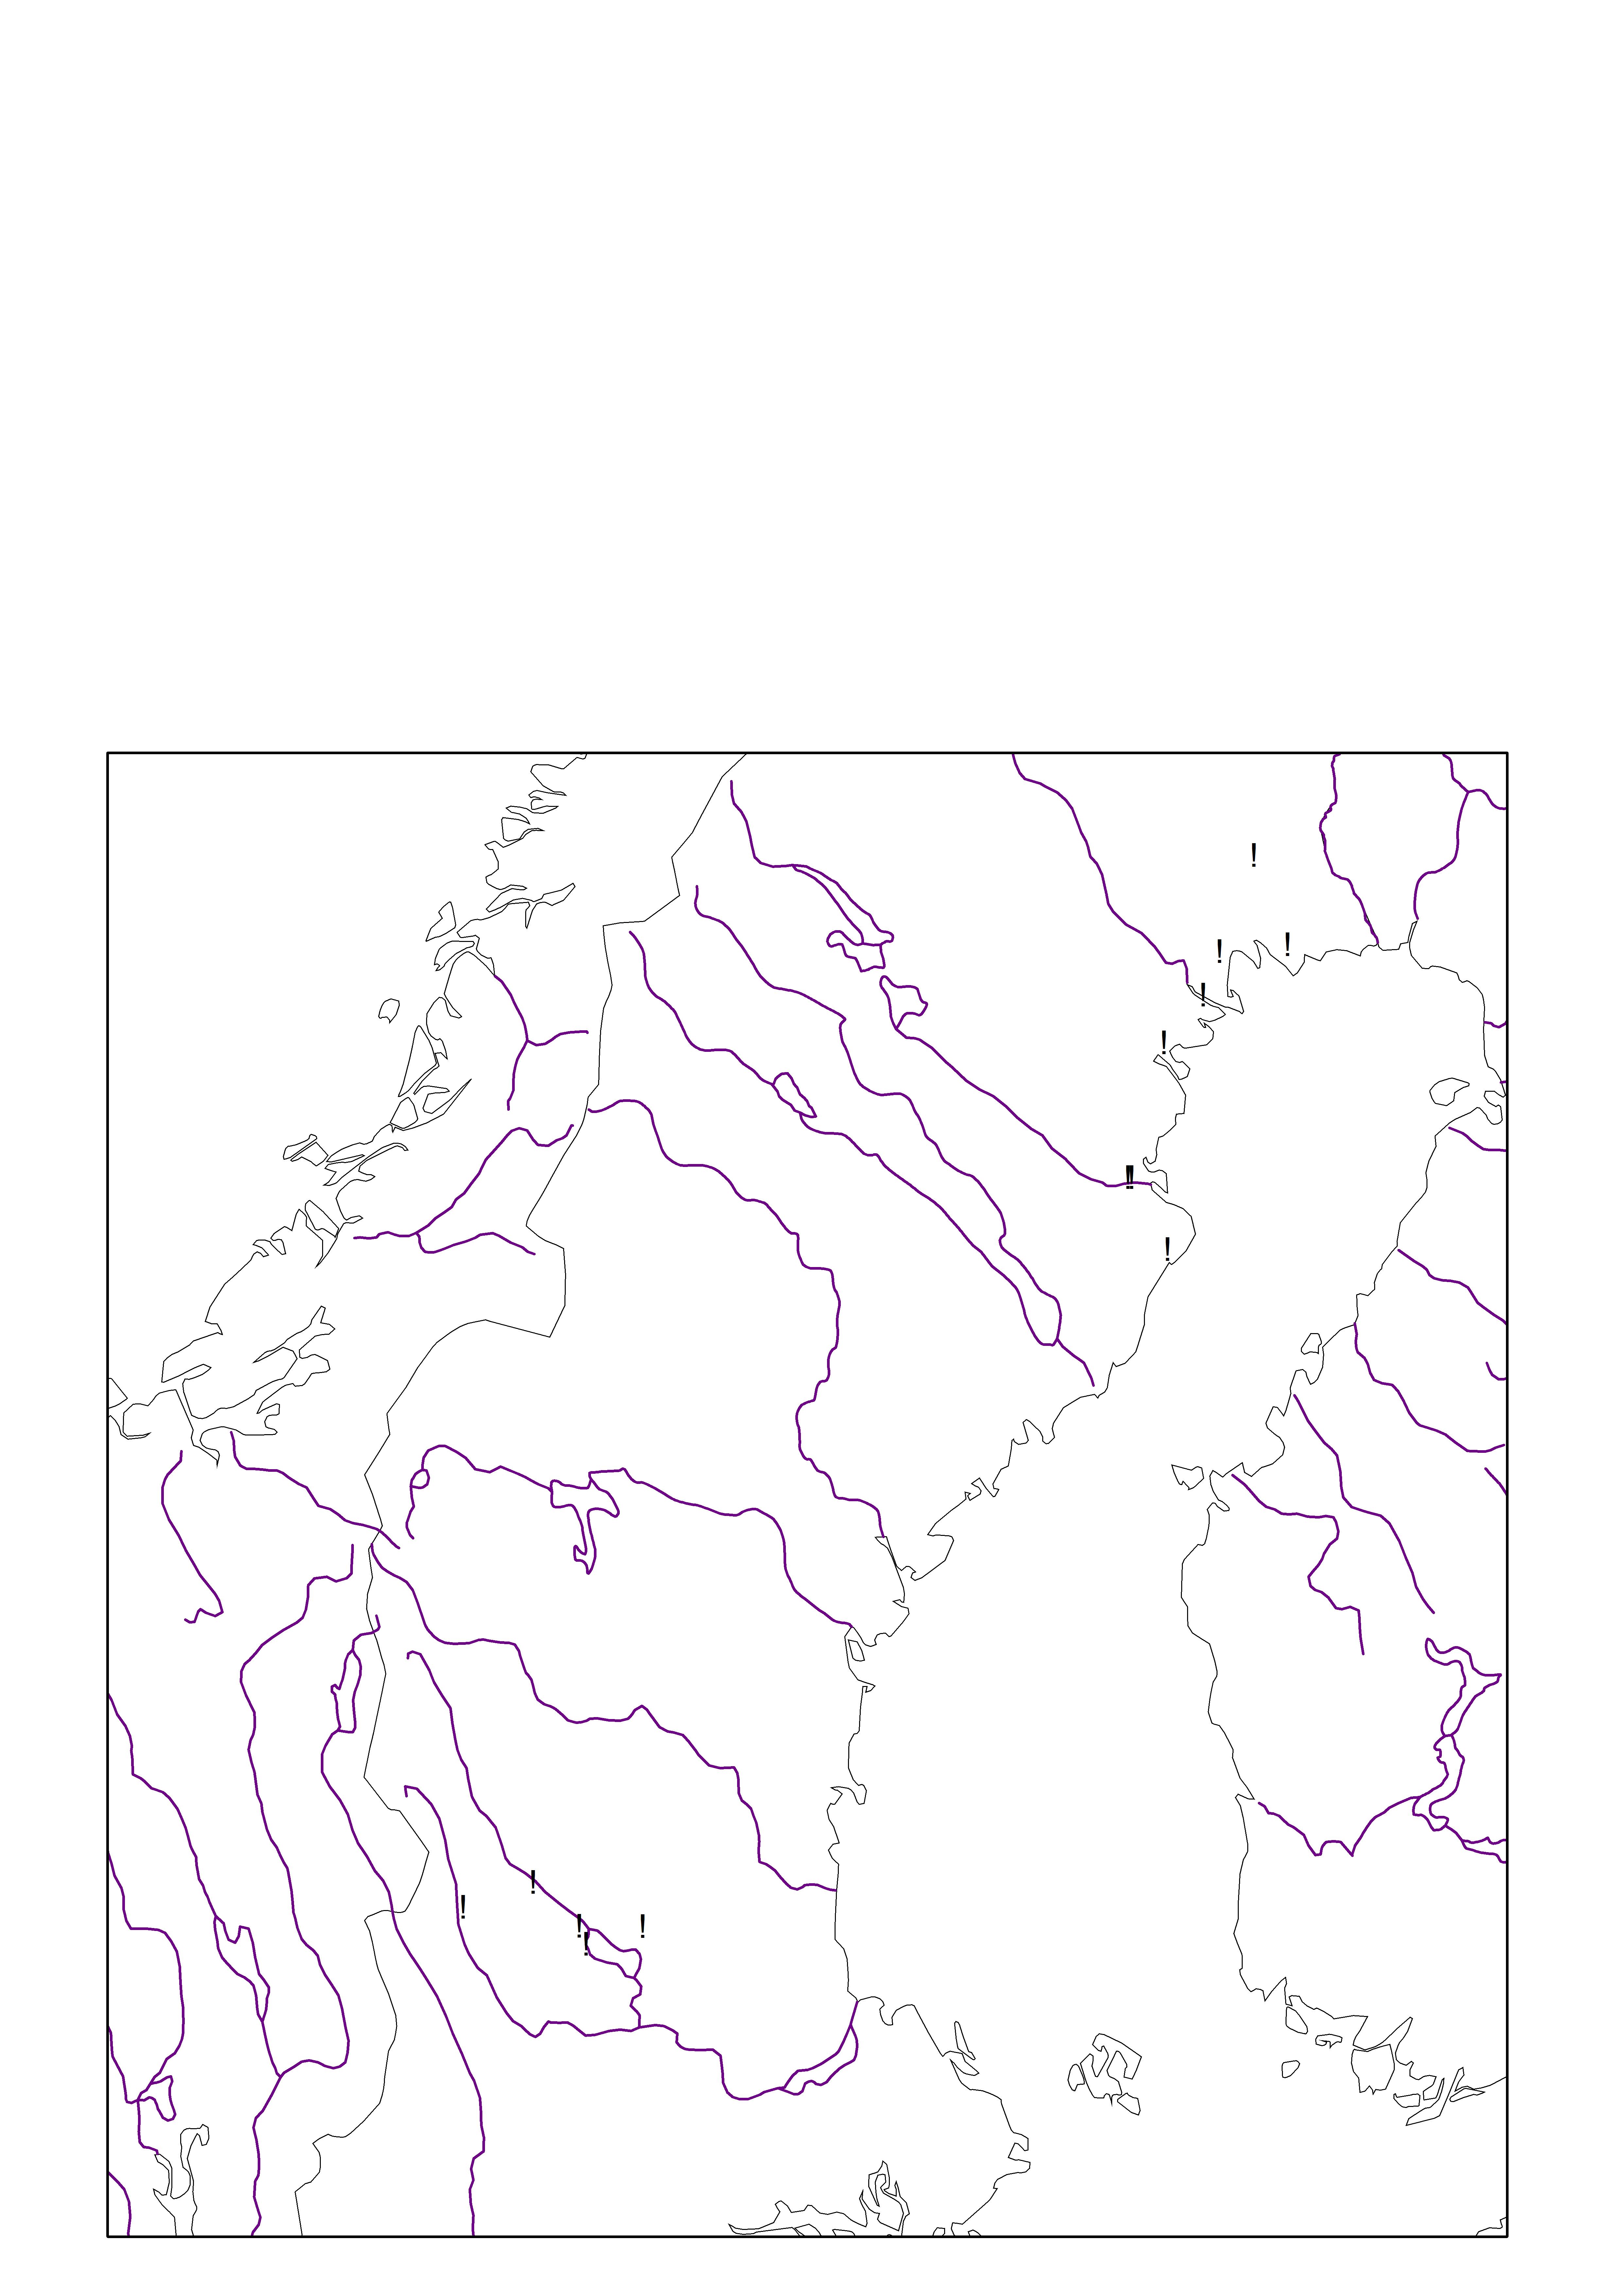
\includegraphics[height=.5\textheight]{figures/22_Attestationsoftheplain}
\caption{Attestations of the plain dative possessive construction.}
\label{map:18}

\end{figure}

\begin{figure}[h]
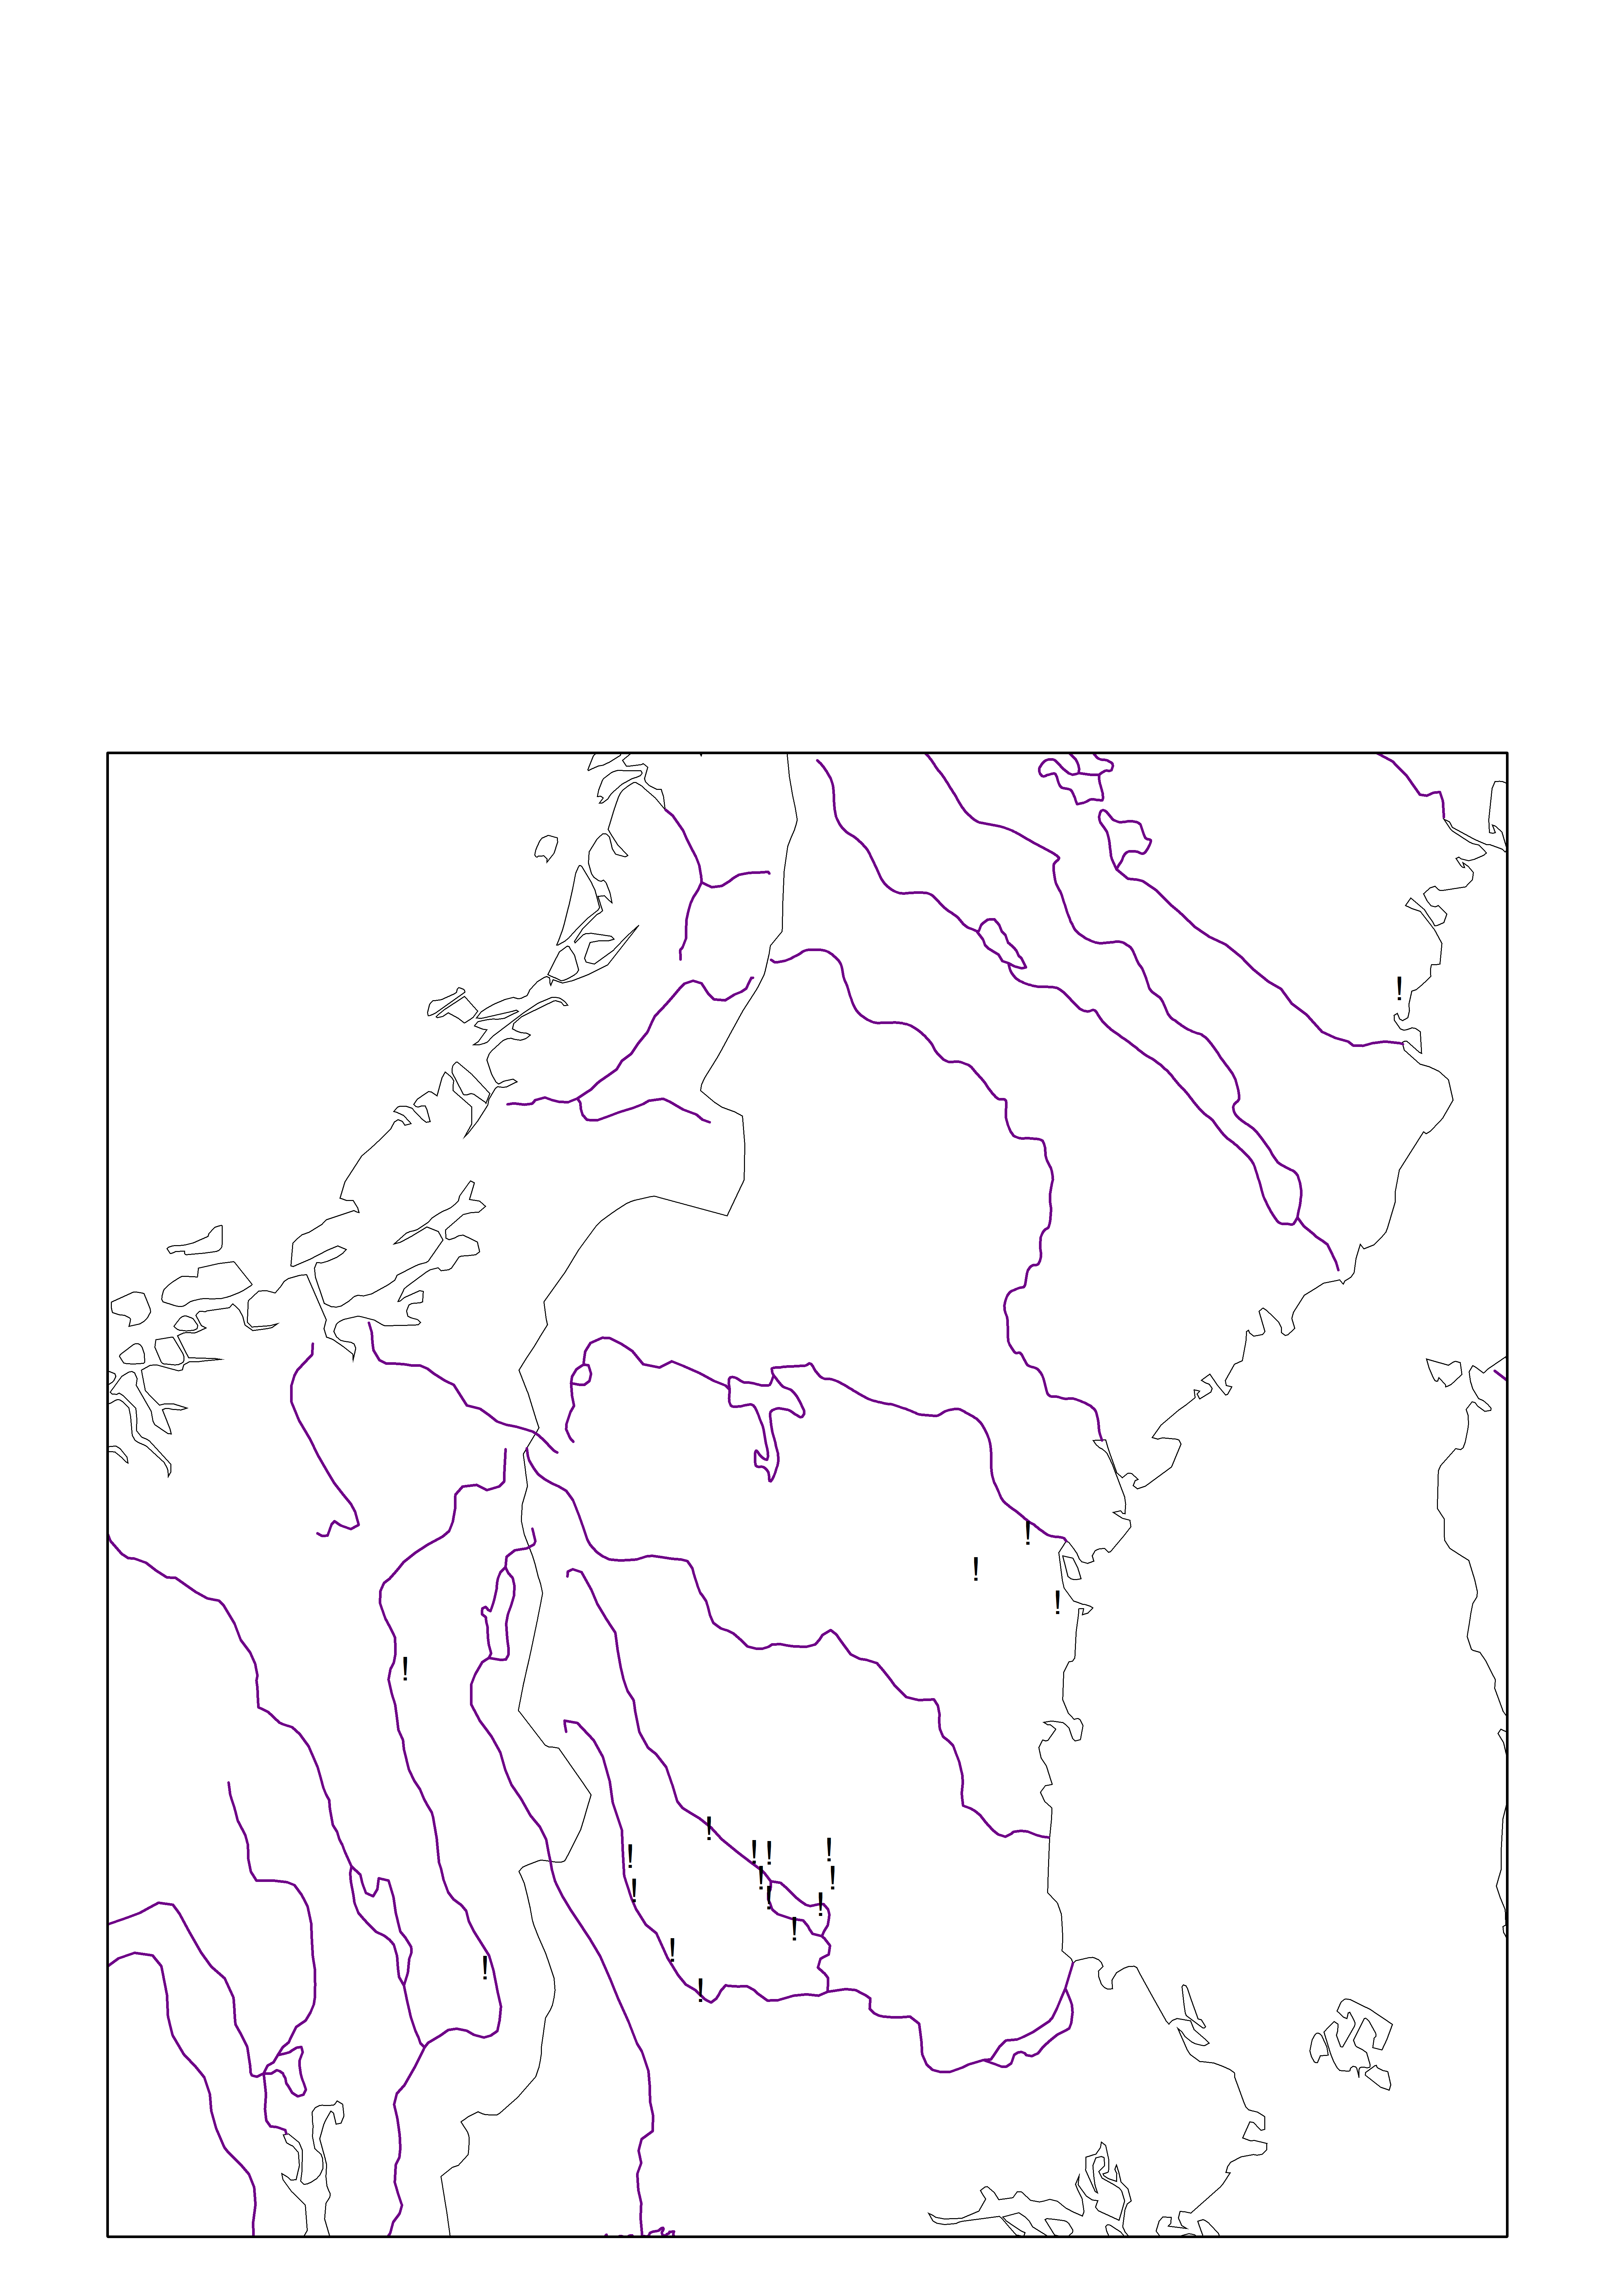
\includegraphics[height=.5\textheight]{figures/23_Attestationsofthecomplex}
\caption{Attestations of the complex dative possessive construction.}
\label{map:19}

\end{figure}

\subsection{The complex dative possessive}
\label{sec:5.4.2}

The dative-marking constructions that we have spoken of so far involve a straightforward combination of a possessee noun with a dative-marked possessor. Another possibility, which I shall refer to as \textbf{the complex dative possessive,} is productive only in Dalecarlian, notably in Elfdalian. The construction I am referring to is superficially quite similar to the Swedish \textstyleLinguisticExample{s}{}-genitive, and is also treated as a kind of genitive construction by \citet{Levander1909}. Let us thus look at his treatment of the genitive in Elfdalian.

According to Levander, all the traditional four cases of Germanic — nominative, genitive, dative, and accusative are found in Elfdalian. However, Levander himself notes that the genitive is fairly rare, especially in the indefinite, where it is basically restricted to two kinds of lexicalized expressions, viz. 

\begin{itemize}
\item after the preposition \textit{et} ‘to’, in expressions such as \textit{et bys} ‘to the village’, \textit{et messer} ‘to the mass’, \textit{et buðer} ‘to the shielings’
\item after the preposition \textit{i} ‘in’, in expressions of time such as \textit{i wittres} ‘last winter’, \textit{i kwelds }‘yesterday evening’
\end{itemize}

%\end{styleAufzhlungszeicheniii}

%\end{listLFOxiiileveli}

%\begin{styleTextkrper}
In these uses, the genitive preserves the original endings (\textit{\nobreakdash-s }in masculine and neuter singular; \nobreakdash-\textit{er} in feminine singular and generally in the plural). This is not the case for the definite forms. Consider the following example (\citet[96]{Levander1909}):

%\end{styleTextkrper}

\ea\label{}
\langinfo{Älvdalen (Os)}{}{}\\
\gll Ita  jar  ir  \textbf{kullum-es} \textbf{saing}.\\
this  here  be.{\prs}  \textbf{girl.{\def}.{\pl}.{\dat}-{\poss}} \textbf{bed}\\
\glt ‘This is the girls’ bed.’
\z

We would expect to find here something like \textstyleLinguisticExample{*kuller }but instead\textstyleLinguisticExample{ }we have something that looks like the dative plural form \textstyleLinguisticExample{kullum} followed by an ending \nobreakdash-\textstyleLinguisticExample{es}. This kind of formation is in fact perfectly general. Thus, we get examples such as \textstyleLinguisticExample{smiðimes} ‘the black-smith’s’, where \nobreakdash-\textstyleLinguisticExample{es }is added to the dative singular definite form \textstyleLinguisticExample{smiðim} of \textstyleLinguisticExample{smið} ‘black-smith’. Further examples:

\ea\label{}
\langinfo{Älvdalen (Os)}{}{}\\
	\ea
		\gll An-dar  skuägen  ir  \textbf{bym-es}.\\
			that  forest.{\def}  be.{\prs}  \textbf{village.{\def}.{\dat}-{\poss}}\\
		\glt ‘This forest belongs to the village.’
	\ex
		\gll Isn-jär  byggnan  ir  \textbf{sån-es}.\\
		this  building.{\def}  be.{\prs}  \textbf{saw-mill.{\def}.{\dat}-{\poss}}\\
		\glt  ‘This building belongs to the saw-mill.’
	\z
\z 

Moreover, as Levander notes, the \nobreakdash-\textstyleLinguisticExample{es} ending may be added to the last word in a complex noun phrase, in which case the possessor noun will still be in the dative:

\ea 
\langinfo{Älvdalen (Os)}{}{}\\
	\ea {
		\gll Ann\footnotemark{}  upp  i  budum-es etta \\
		Anna.{\dat}  up  in  shieling.{\dat}.{\pl}-{\poss}  hood\\
		\glt ‘Anna-at-the-shieling’s hood’ 
	}
	\ex {
		\gll An  bar  \textbf{pridikantem} \textbf{jär} \textbf{upp-es} an. \\
		he  carry.PRET  \textbf{preacher.{\def}.{\dat}.{\sg}} \textbf{here} \textbf{up-{\poss}} he\\
		\glt ‘He carried the stuff of the preacher’s [stuff] up here, he did.’
	}
	\z
\z 

\footnotetext{The dative form of \textit{Anna} is given by Levander as \textit{Anno} but the final vowel is elided here due to the morphophonological process known as apocope (see further in the main text).}

(In (b), the possessive noun phrase is headless, i.e. the possessee is implicit.) 

Indeed, if the possessor is expressed by a noun phrase determined by a possessive pronoun,\textit{ {}-}\textstyleLinguisticExample{es} is added directly to that noun phrase, with the possessive pronoun in the dative case:

\ea\label{}
\langinfo{Älvdalen (Os)}{}{}\\
\ea {
\gll Is\k{u}  jär  lodǫ  ar  stendeð ǫ  \textbf{mainum} \textbf{faðer-es } \textbf{garde.} \\
this.{\f}.{\sg}.{\nom}  here  barn.{\def}.{\nom}.{\sg}  have.{\prs}.{\sg}  stand.{\sup} on  \textbf{my.{\m}.{\sg}.{\dat}} \textbf{father-{\poss}} \textbf{farm.{\dat}.{\sg}} \\
\glt ‘This barn has stood on my father’s farm.’
}
\ex {
\gll Eð  war  \textbf{uorum} \textbf{fafar-es} \textbf{fafar} so  byggd  dǫ  dar  tjyälbuðe;.\footnotemark{}\\
it  be.PRET.{\sg}  \textbf{our.{\m}.{\dat}.{\sg}.} \textbf{father’s\_father-{\poss}} \textbf{father’s\_father} who  build.PRET  that.{\f}.{\sg}.{\acc}  there  shelter.{\def}.{\acc}.{\sg}\\
\glt ‘It was our great-great-great-grandfather who built that shelter.’
}
\ex {
\gll Eð  war  \textbf{dainum} \textbf{kall-es} \textbf{mumun.}\\
it  be.PRET.{\sg}  \textbf{your.{\m}.{\dat}.{\sg}.} \textbf{husband-{\poss}} \textbf{mother’s\_mother}\\
\glt ‘It was your husband’s maternal grandmother.’
}
\z 
\z

\footnotetext{This word, which translates into regional Swedish as\textit{ (myr)slogbod}, denotes a structure somewhat similar to a bus stop shelter used during activities in remote places such as hunting, fishing and hay-harvesting.}

The marker\textit{ {}-}\textstyleLinguisticExample{es} can also be added to headless adjectives with a definite suffix (see \sectref{sec:4.7}) and some pronouns:

\ea\label{}
\langinfo{Älvdalen (Os)}{}{}\\
\ea {
\gll Oðra;  ir  \textbf{ljuätam-es.}\\
other.{\def}.{\f}.{\sg}  be.{\prs}  \textbf{evil.{\def}.{\m}.{\dat}-{\poss}}\\
\glt ‘The other one belongs to the Evil One.’
}

\ex {
\gll Ermkläd  ir  \textbf{dumbun-es.}\\
scarf.{\def}  be.{\prs}  \textbf{dumb.{\def}.{\f}.{\dat}-{\poss}}\\
\glt ‘The scarf belongs to the deaf-and-dumb woman.’\footnotemark{}
}

\ex {
\gll Eð  ir  \textbf{ingumdier-es} \textbf{stjäl} min.  \\
it  be.{\prs}  \textbf{neither.{\dat}.{\m}.{\sg}-{\poss}} \textbf{reason} with  \\
\glt ‘There is no reason for either one.’
}
\z 
\z

\footnotetext{The feminine ending of the adjective indicates that the referent is a woman.}

It seems that there is a recent increase in the frequency of the \nobreakdash-\textstyleLinguisticExample{es} construction in modern Elfdalian, which is most probably due to it being seen as the closest equivalent of the Swedish \textstyleLinguisticExample{s}{}-genitive. An interesting phenomenon in this connection is the tendency for native speakers to make \textstyleLinguisticExample{es} a separate word in written Elfdalian (or sometimes hyphenated, as in \textstyleLinguisticExample{bil-es stor} ‘uncle’s walking-stick’). Perhaps most strikingly, \textstyleLinguisticExample{es} is even used after a preceding vowel, although, due to extensive apocope, hiatus is not a common phenomenon in Elfdalian. Consider a proper name such as \textstyleLinguisticExample{Anna}, for which Levander gives the dative form \textstyleLinguisticExample{Anno} and the “genitive” \textstyleLinguisticExample{Annes}, the latter being the logical outcome of apocopating the dative form before {}-\textstyleLinguisticExample{es}. In modern Elfdalian, however, proper names in\textit{ {}-a}\textstyleLinguisticExample{ }are normally treated as undeclinable and are shielded against apocope. Thus ‘Anna’s book’ comes out as \textstyleLinguisticExample{Anna es buäk}. 

The tendencies mentioned in the previous paragraph come out very clearly in one of the few longer texts written in Elfdalian, [S21], where the complex dative construction is the most frequent way of expressing nominal possession, and \textstyleLinguisticExample{es} is fairly consistently written separately. There are several examples where the preceding noun ends in a vowel such as \textstyleLinguisticExample{Kung Gösta es dågå} ‘King Gösta’s days’ and \textstyleLinguisticExample{Sparre es klauter} ‘Sparre’s clothes’. Whereas proper names are generally not case-marked, most definite possessor nouns are in the dative, but there are also examples of nominative possessor preceding \textstyleLinguisticExample{es}. ([S21] is on the whole heavily influenced by Swedish – there are also a fair number of literal transfers of \textstyleLinguisticExample{s}{}-genitives, such as\textstyleLinguisticExample{ Luthers katitsies} ‘Luther’s catechesis’.) Compare \REF{280}, where the nominative form \textstyleLinguisticExample{prestsaida} ‘the clergy side’ is used rather than the dative \textstyleLinguisticExample{prestsaidun}:

\ea\label{}
\langinfo{\label{bkm:Ref135470135}Älvdalen (Os)}{}{}\\
\gll Nu  war  ed  \textbf{prestsaida} \textbf{es} \textbf{tur} at  tytts at  muotstonderer  språked  um  nǫd  eller  eld  ed dier  uld  tag  stellning  ad  ǫ  stemmun.\\
now  be.{\pst}  it  \textbf{clergy-side.{\def}} \textbf{{\poss}} \textbf{turn} {\infm}  think.{\inf}that  adversary.{\def}.{\pl}  speak.{\pst}  about  something  other  than  it they  shall.{\pst}  take.{\inf} position  to  on  meeting.{\def}.{\dat}\\
\glt ‘Now it was the turn of the clergy side to think that the adversaries were talking about something other than what should be decided at the meeting.’ 
\z

The construction \textstyleLinguisticExample{eð ir NP es tur at V-inf} ‘it is NP’s turn to V’ is calqued quite directly on the corresponding Swedish construction \textstyleLinguisticExample{det är NPs tur att V-inf}, but seems to have been firmly entrenched in Elfdalian for quite some time. Compare the following example from a speaker born in the 1850’s:

\ea\label{}
\langinfo{\label{bkm:Ref135470154}Älvdalen (Os)}{}{}\\
\gll …å  se  vart  ed  \textbf{bumuą̈r} \textbf{es} \textbf{tur}\\
and  then  become.{\pst}  it  \textbf{shieling hostess} \textbf{{\poss}} \textbf{turn}\\
\gll tä  tag  riäd   o  mjotsin\\
to  take.{\inf} care  about  milk.{\def}.{\dat}\\
\gll da  gesslkallär  ad  fer  ad  raisą̈.\\
when  herder\_boy.{\pl}  have.{\pst}  go.{\sup}  to  forest.{\def}.{\dat}\\
\glt ‘…and then it was the shieling hostess’s turn to take care of the milk when the herder boys had gone to the woods.’ [S16]
\z

Here, however, the noun form \textstyleLinguisticExample{bumuą̈r} ‘shieling hostess’ is ambiguous between nominative and dative. Notice also that whereas the infinitive marker in \REF{280} is the Swedish-inspired \textstyleLinguisticExample{at}, \REF{281} has the more genuine Elfdalian \textstyleLinguisticExample{tä} (see \sectref{sec:6.4.1}). 

Much of what has been said about the Elfdalian construction carries over to other Ovansiljan varieties. According to \citet[170]{Levander1928}, “definite genitive forms” formed by adding a suffix to the definite dative singular are found in most Dalecarlian varieties where the dative is preserved. In Ovansiljan (except Orsa) and Nedansiljan, the suffix is\textit{ {}-s} preceded by some vowel whose quality varies between \textstyleLinguisticExample{e, å, ä, a,} and \textstyleLinguisticExample{ô}. In Västerdalarna and Orsa, the suffix is simply\textstyleLinguisticExample{ {}-s}, except in Äppelbo, where it is\textstyleLinguisticExample{ {}-säs}. Examples can also be found in modern texts. Consider the following example from Mora:

\ea\label{}
\langinfo{Östnor, Mora (Os)}{}{}\\
\gll Welsignarn  e  an\\
blessed  be.{\prs}  he\\
\gll så  kum  i  \textbf{Ärram-ås} \textbf{nammen!}\\
who  come.{\prs}  in  \textbf{Lord.{\def}.{\dat}-{\poss}} \textbf{name}\\
\glt ‘Blessed is he who comes in the name of the \href{http://www.godrules.net/library/topics/topic1192.htm}{Lord}!’ (Matthew 21:9) [S20]
\z

In \textstyleLinguisticExample{Ärram-ås,} the suffix\textit{ {}-å}\textstyleLinguisticExample{s} has been added to the definite dative form \textstyleLinguisticExample{Ärram. }In texts from other villages, however,\textit{ {}-å}\textstyleLinguisticExample{s} is also sometimes added to the nominative:

\ea\label{}
\langinfo{Utmeland, Mora (Os)}{}{}\\
\gll Då  stod  \textbf{Ärran-ås} \textbf{angel} framåmin  dem…\\
then  stand.{\pst}  \textbf{Lord.{\def}-{\poss}} \textbf{angel} in front of  they.{\obl}\\
\glt ‘And then the angel of the Lord stood before them…’ (Luke 2:9) [S20]
\z

In the following example, the suffix is added to a postposed possessive pronoun:

\ea\label{}
\langinfo{\textit{Önamål} (Hökberg, Mora, Os)}{}{}\\
\gll Wennfe  si  du  twårpär  i  \textbf{bror} \textbf{denås} \textbf{öga…}\\
why  see.{\prs}  you  speck.{\pl}  in  \textbf{brother} \textbf{your-{\poss}} \textbf{eye}\\
\glt ‘And why do you see specks in your brother’s eye…’ (Matt. 7:3) [S20]
\z

In other village varieties in Mora, the possessive pronoun is preposed and we get \textstyleLinguisticExample{den brorås.}

In Sollerön, according to \citet[357]{AnderssonEtAl1999}, the suffix\textit{ {}-a}\textstyleLinguisticExample{s} is added to the dative, or in modern varieties of the vernacular, to the nominative: \textstyleLinguisticExample{donda kallimas kelingg} or \textstyleLinguisticExample{donda kallnas kelingg} ‘that man’s wife’. Proper names in\textit{ {}-a} such as \textstyleLinguisticExample{Anna} have genitive forms such as \textstyleLinguisticExample{Annonas }(but in a questionnaire from Sollerön \textstyleLinguisticExample{Annaas} is given as an alternative).

There is also some sporadic evidence of similar constructions outside of Dalecarlian. Thus, \citet[124]{Larsson1929} quotes an unpublished description of the vernacular of Byske (NVb), Lundberg (n.y.), as mentioning “a genitive with an \textstyleLinguisticExample{s} added to the dative form, in the same way as in Dalecarlian”, e.g. \textstyleLinguisticExample{pajkoms} ‘the boy’s, the boys’’, \textstyleLinguisticExample{sanoms} ‘the son’s’, \textstyleLinguisticExample{sönjoms} ‘the sons’’, \textstyleLinguisticExample{kooms} ‘the cow’s, the cows’, but claims that no such form has been attested by later researchers (including himself). However, Larsson adds: when questioned directly, informants confirm that \textstyleLinguisticExample{s} can added to dative of masculines “in independent position”, e.g. \textstyleLinguisticExample{he jer gobboms} ‘it is the old man’s’. 

\citet[126]{Hellbom1961} quotes Larsson and says that “similar constructions seem to have existed also in Medelpad, above all when a preposition precedes the genitive”.\footnote{ “Likartade bildningar ser ut att ha förekommit även i Medelpad, främst då när en prep. föregått genitiven.”} Medelpad is otherwise an area where the dative had already virtually disappeared at the end of the 19\textsuperscript{th} century. Hellbom’s first example is from Njurunda, his own native parish. The text, however, was already written down in 1874:

\ea\label{}
\langinfo{\label{bkm:Ref126396484}Njurunda (Md)}{}{}\\
\gll Hæ  var  en  tå  \textbf{ryssôm-s} \textbf{vaktknekter}\\
it  be.{\pst}  one  of  Russian.{\pl}.{\dat}-{\poss}  sentinel.{\pl}\\
\gll sôm  hadde  sômne  åv  å  låg  å  snarke.\\
who  have.{\pst}  fall\_asleep.{\sup}  off  and  lie.{\pst}  and  snore.{\pst}\\
\glt  ‘It was one of the Russians’ sentinels who had fallen asleep and lay snoring.’ [S38]
\z

Here, there is indeed a dative-governing preposition before the possessive construction. If this were an isolated example, we would probably interpret the form \textstyleLinguisticExample{ryssôms} as resulting from a confusion of two syntactic structures. (\citet[38]{Delsing2003a} mentions \REF{285} as an example of a “group genitive”, which, however, presupposes the less likely interpretation ‘a sentinel of one of the Russians’ rather than ‘one of the Russians’ sentinels’.) 

Hellbom (ibid.) quotes an unpublished note by Karl-Hampus Dahlstedt to the effect that some people in the parish of Indal in the province of Medelpad used the form \textstyleLinguisticExample{bånôms} in the genitive plural of \textit{bån} ‘child’. He also enumerates a few examples of forms where the genitive\textstyleLinguisticExample{ {}-s} is added to what looks like an oblique form of a weak noun, which at older stages of the language was ambiguous between genitive, dative, and accusative: \textstyleLinguisticExample{fårsjinnpälsa gubbas} ‘the old man’s sheep fur coat’; \textstyleLinguisticExample{gu{\textasciigrave}bbass bökksan} ‘the old man’s trousers’; \textstyleLinguisticExample{ti gu{\textasciigrave}bbass kammarn} ‘to the old man’s chamber’. His final example, however, is somewhat more spectacular,\footnote{ “Slutligen ett mera tillspetsat belägg från Stöde 1877”} in that it appears to exemplify the addition of the genitive\textstyleLinguisticExample{ {}-s} as a phrasal clitic to an NP in the dative. 

\ea\label{}
\langinfo{Stöde (Md)}{}{}\\
\gll in  par  jänter  …  som  fôǠDǠDe  mä\\
{\indf}  couple  girl.{\pl}.{\dat}    who  follow.{\pst}  with\\
\gll på  \textbf{fara} \textbf{senne-}\textbf{\textit{  }}\textbf{\textit{\nobreakdash-s}} \textbf{joLsättning} \\
on  \textbf{father.{\dat}} \textbf{their.{\refl}.{\dat}} \textbf{{\poss}} \textbf{funeral} \\
\glt ‘…a couple of girls … who took part in their father’s funeral.’ [S15]
\z

Genitive forms where the\textstyleLinguisticExample{ {}-s} is added to an oblique form of a weak noun are quite common in Medieval Scandinavian. (Recall that weak masculine nouns had a single form for genitive, dative and accusative in the singular.) A form such as \textstyleLinguisticExample{bondans} ‘the farmer’s’ is actually fairly straightforwardly derivable from something like \textstyleLinguisticExample{bonda hins}. In other forms, we have to assume an extension by analogy of this formation, as in \textstyleLinguisticExample{kirkionnes} ‘of the church’ instead of the older \textstyleLinguisticExample{kirkionnar} (Wessén (1968: I:143)). The Medelpadian \textstyleLinguisticExample{gubbas} could be interpreted in the same way, although it might perhaps also be derivable from an older \textstyleLinguisticExample{gubbans}. A genitive ending\textit{ {}-a}\textstyleLinguisticExample{s} is in fact found in various vernaculars. In Vätö (Uppland), as described by \citet{Schagerström1882}, weak stem proper names take the endings\textit{ {}-a}\textstyleLinguisticExample{s} (masc.) and \nobreakdash-\textstyleLinguisticExample{ôs} (fem.). In Ostrobothnian,\textit{ {}-a}\textstyleLinguisticExample{s} as a genitive ending can be added to the definite form of masculine common nouns, such as \textstyleLinguisticExample{rävinas} ‘of the fox’ and \textstyleLinguisticExample{varjinas} ‘of the wolf’. This is a more radical extension than what we find in Vätö, since in these forms there is no historical motivation for the \textstyleLinguisticExample{a} vowel. In these cases, on the other hand, there is no connection to the dative case, which has been wholly lost in Ostrobothnian. However, there is an intriguing parallel to the Dalecarlian construction. \citet[43]{ErikssonEtAl1999} found a variation among their Ostrobothnian informants between\textstyleLinguisticExample{ {}-s} and\textit{ {}-a}\textstyleLinguisticExample{s} as a genitive or possessive marker, with a possible concentration of\textit{ {}-a}\textstyleLinguisticExample{s} in the southern part of the province. The general pattern was for the\textit{ {}-a}\textstyleLinguisticExample{s} marker: possessor noun +\textit{ {}-a}\textstyleLinguisticExample{s} + possessee + definite suffix. In two of the examples in the questionnaire, the possessor noun was the proper name \textstyleLinguisticExample{Anna. }Here, “the informants felt forced to mark an orthographic boundary”, yielding spellings such as \textstyleLinguisticExample{Anna’as haanden} ‘Anna’s hand’ and \textstyleLinguisticExample{Anna as gamlest systren }‘Anna’s eldest sister’, which closely parallel the Elfdalian forms quoted above (except for the definite form of the head noun).

In his discussion of the confusion between the dative and the genitive in Medieval Norwegian, \citet{Larsen1895} mentions a few examples which look like complex dative possessives, for instance in this document from Rendalen in 1546:

\ea\label{}
\langinfo{Rendalen (Hedmark, Norway, 16\textsuperscript{th} century)}{}{}\\
\gll …med  …  theyriss  \textbf{bondomss} Karls  Jonsszon\\
…with    their  \textbf{husband.{\dat}.{\pl}-{\poss}} Karl.{\gen}  Jonsszon\\
\gll Engilbrictz  Asmarsszon  oc  Trondz  Eyriksszon\\
Engilbrict.{\gen}  Asmarsszon  and  Trond.{\gen}   Eyriksszon\\
\gll oc  theyriss  \textbf{barnomss}  godom  vilie…\\
and  their  \textbf{child.{\dat}.{\pl}-{\poss}} good.{\dat}.{\sg}.{\m}  will..\\
\glt ‘…with the good will of their husbands Karl Jonsson Engelbrikt Asmarsson and Trond Eyriksson and their children…’
\z

In addition, he mentions that in the Norwegian Solør vernaculars where the dative is still preserved, the construction \textstyleLinguisticExample{for NP’s skull }‘for NP’s sake’ commonly employs genitives formed from the dative, as in \textstyleLinguisticExample{for gutas (jintns, bånis, ongoms) skull} ‘for the boy’s (girl’s, child’s, kids’) sake’. 

Returning to the complex dative possessive in Elfdalian, we can see that it has a number of specific properties: (i) there is a general syllabic marker \textstyleLinguisticExample{(-)es}; (ii) the marker is combined with a dative form of the possessor; (iii) the marker has the character of a clitic added to a full noun phrase rather than an affix added to a noun. The last point is supported by  the following facts: (a) modifiers of the possessor NP are in the dative (at least in more conservative forms of the language); (b) the vowel of the marker is not elided after nouns ending in vowels; (c) the marker is placed on the last word of an NP rather than on the head noun; and (d) native speakers tend to write the marker as a separate word. In the Peripheral Swedish area outside Dalecarlian, we find sporadic examples of possessive constructions that share some of these properties but hardly any that have all of them. In fact, with respect to (iii) there are also parallels with the \textstyleLinguisticExample{s}{}-genitive of Central Scandinavian and English. 

What can we say about the possible evolution of the complex dative construction? 

The geographically quite dispersed although sporadic and rather heterogeneous manifestations suggest that the construction was more widespread earlier. It is likely that the general demise of the dative has made it either disappear or be transformed. We may note that the examples from modern Elfdalian suggest that \textstyleLinguisticExample{(-)es }now tends to be added to a noun phrase that has no case-marking, and that is also the case for the Ostrobothnian examples. It is also possible that the tendency to treat \textstyleLinguisticExample{es} as a clitic with no influence on the form of the previous word is a relatively recent phenomenon in Elfdalian.  

The most natural approach to the genesis of the complex dative construction would \textit{prima facie} be to try and explain it as a result of a development similar to that described for the \textstyleLinguisticExample{s}{}-genitive by e.g. \citet{Norde1997}, that is, by a “degrammaticalization” of the genitive \textstyleLinguisticExample{s-}ending of early Scandinavian. After the introduction of suffixed articles, the \textstyleLinguisticExample{s-}ending was found in indefinite masculine and neuter singular strong nouns and in all definite masculine and neuter singulars. Later on, it spread to other paradigms, and was then typically grafted on to the old genitive forms. If these were non-distinct or similar to the dative forms, it is possible that they were reanalyzed as such, which could have triggered a generalization of the pattern dative + \textstyleLinguisticExample{s-}ending. Such a hypothesis is not unproblematic, however. If we suppose that the source of the Elfdalian \textstyleLinguisticExample{uksa-m-es} ‘of the ox’ is a medieval Scandinavian form such as \textstyleLinguisticExample{oksa-ns} ‘ox.{\def}.{\gen}.{\sg}’, we have to assume that the apparent dative form of the stem would trigger the choice of a dative definite suffix, and we also have to explain where the vowel in the suffix comes from. 

One peculiar circumstance around the complex dative possessive is that its functional load was apparently rather small in the pre-modern vernaculars where it existed. We have seen that there are only very sporadic examples from the Norrlandic dialects, and even in Elfdalian around 1900 it was, according to \citet[98-99]{Levander1909}, “rare”,\footnote{ “Bestämd genitiv är likaledes sällsynt…”} the simple dative possessive being the preferred alternative (On the other hand, this claim is in a way contradicted by the fact that Levander himself provides no fewer than 17 examples of the complex dative construction in his grammar.) 

Why was it, then, kept in the language at all? One possible explanation is that the complex dative possessive had a specialized function. Something that speaks in favour of this is that a surprisingly large number of the examples quoted in the literature from older stages of the vernaculars displays the possessive NP in predicate position. This goes for the only example that Larsson quotes as still acceptable to his informants from Byske in Västerbotten, and out of Levander’s 17 examples, 12 directly follow a copula. It is also striking that ten of these are headless – which parallels Larsson’s claim that the complex dative construction is allowable “in independent position”. We might thus hypothesize that the complex dative possessive developed as an alternative to the simple dative possessive primarily in predicate position and/or when used without a head noun. 

If we look around in the Germanic world, the constructions discussed in this section are not without their parallels. Consider the following examples: 

\ea\label{}
\langinfo{\label{bkm:Ref126571184}Middle English (13\textsuperscript{th} century)}{}{}\\
\gll of  Seth  ðe  was  \textbf{Adam} \textbf{is} \textbf{sune}\\
of  Seth  who  be.{\pst}  \textbf{Adam} \textbf{{\poss}} \textbf{son}\\
\glt ‘of Seth, who was Adam’s son’ [S3]
\z

\ea\label{}
\langinfo{\label{bkm:Ref151373829}Middle Dutch}{}{}\\
\gll Grote  Kaerle  sijn  soon\\
Great.{\dat}  Charles.{\dat}  his  son\\
\glt ‘great Charles’ son’
\z

\ea\label{}
\langinfo{Dutch}{}{}\\
\gll Jan  z’n  boek\\
Jan  {\poss}   book\\
\glt ‘Jan’s book’
\z

\ea\label{}
\langinfo{\label{bkm:Ref151373831}Afrikaans }{}{}\\
\gll Marie  se  boek\\
Mary  {\poss}  book\\
\glt ‘Marie’s book’ (\REF{289}{}-\REF{291} quoted from \citet[56]{Norde1997})
\z

Following Koptjevskaja-\citet{Koptjevskaja-Tamm2003, we can call these constructions \textbf{linking pronoun possessives}. In the most elaborated type, exemplified here by Middle Dutch, they contain a possessive pronoun between the case-marked possessor noun phrase and the head noun. In the Middle Dutch example \REF{289}, the possessor noun is in the dative case,\footnote{ This analysis is questioned in \citet{Allen2008}.} as it is in the following Modern German title of a best-selling book on German grammar (\citet{Sick2004}):

\ea\label{}
\langinfo{\label{bkm:Ref126571195}German}{}{}\\
\gll Der  Dativ  ist  \textbf{dem} \textbf{Genitiv} \textbf{sein} \textbf{Tod}\\
{\def}.{\m}.{\sg}.{\nom}  dative  be.{\prs}  \textbf{{\def}.{\m}.{\sg}.{\dat}} \textbf{genitive} \textbf{{\poss}.{\m}.{\sg}.{\nom}} \textbf{death}\\
\glt  ‘The dative is the death of the genitive.’
\z

 However, genitive possessor nouns are also attested in Middle Dutch/Low German:

\ea\label{}
\langinfo{Middle Dutch}{}{}\\
\gll alle  des  konincks  sijn  landen\\
all  {\def}.{\m}.{\gen}  king.{\gen}  his  land.{\pl}\\
\glt ‘all the king’s lands’ (\citet[58]{Norde1997})
\z

In Germanic varieties where the dative case is no longer alive, e.g. Middle English, Modern Dutch and Afrikaans, the possessor NP in linking pronoun possessives has no case marking (cf. \REF{288}{}-\REF{292}). In Afrikaans, we can also see that the linking morpheme \textstyleLinguisticExample{se} has been differentiated in form from the masculine possessive \textstyleLinguisticExample{sy} and has been generalized also to feminines (and plurals).

In Scandinavian languages, there are at least two types of linking pronoun constructions. One involves non-reflexive possessive pronouns and was apparently quite common in written Danish from the Late Middle Age on (\citet[61]{Knudsen1941}): \textstyleLinguisticExample{Graamand hans vrede }‘Gramand’s wrath’; \textstyleLinguisticExample{en enkkæ hennes søn} ‘a widow’s son’. This construction is now only marginally possible in bureaucratic style (Modern Norwegian: \textstyleLinguisticExample{Oasen Grillbar Dets Konkursbo} ‘the insolvent estate of the grill bar \textstyleLinguisticExample{Oasen}’ (Internet)). The construction was often used in cases where a group genitive might be expected in the modern Central Scandinavian, such as \textstyleLinguisticExample{prestens i Midian hans queg} ‘the priest in Midian’s cattle’ (16\textsuperscript{th} century Bible translation). As the last example illustrates, the head noun could also be genitive-marked (according to Knudsen this was relatively uncommon, however). The construction still exists in Jutland, “in particular northern Jutish” (\citet[62]{Knudsen1941}): \textstyleLinguisticExample{æ skrædder hans hus} ‘the tailor’s house’.

The second Scandinavian linking pronoun construction is found in Norwegian (at least originally predominantly in western and northern varieties) and involves reflexive linking pronouns:

\ea\label{}
\langinfo{Norwegian}{}{}\\
\gll mannen  sin  hatt\\
man.{\def}  {\poss}.{\refl}.3{\sg}  hat\\
\glt ‘the man’s hat’
\z

This construction is generally assumed to have arisen under German influence and is therefore traditionally called “garpegenitiv”, \textstyleLinguisticExample{garp} being a derogatory term for ‘German’.

Typological parallels to the Germanic linking pronoun possessives are found, for example, in Ossetian (Iranian; Koptjevskaja-\citet[669]{Koptjevskaja-Tamm2003). One could also see them as the analytic analogue to possessive constructions in which a possessive affix on the head noun agrees with the possessor noun phrase, as in Hungarian:

\ea\label{}
\langinfo{Hungarian}{}{}\\
\gll a  szomszéd  kert-je\\
{\def}  neighbour  garden-3{\sg}.{\poss}\\
\glt ‘the neighbour’s garden’ (Koptjevskaja-\citet[648]{Koptjevskaja-Tamm2003) 
\z

The Germanic linking pronoun possessive constructions are controversial, both with respect to their origin and their possible role in the history of the \textstyleLinguisticExample{s}{}-genitive. They could have originated, as claimed by some scholars, from a reanalysis of an indirect object construction (\citet[638]{Behaghel1923}), such as:

\ea\label{}
\langinfo{German}{}{}\\
\gll Er  hat  \textbf{meinem} \textbf{Vater} \textit{seinen}\textit{  Hut}\textit{  }genommen.\\
he  have.{\prs}  \textbf{my.{\dat}.{\m}.{\sg}} \textbf{father} \textit{his.{\acc}.{\m}.{\sg}}\textit{  }\textit{hat}\textit{  }take.PP\\
\glt ‘He has taken from my father his hat.’?’he has taken my father’s hat.’
\z

Some Dutch scholars, quoted by \citet[58]{Norde1997}, have suggested that the linking pronoun is a “pleonastic addition”, added for clarity. For Middle English, a common view is that the linking pronoun \textstyleLinguisticExample{(h)is} is actually a reanalysis of the old genitive ending.

Independently of what the origin of the linker is, it may or may not have played a role in the development of the English \textstyleLinguisticExample{s}{}-genitive (\citet{Janda1980}). The reanalysis of the \textstyleLinguisticExample{s-}ending as a pronoun could have facilitated the rise of group genitives, where the possessive marker was placed at the end of the noun phrase. \citet[91]{Norde1997} comments on this hypothesis as follows: “Even though this may seem to be a plausible scenario for English, it should be borne in mind that the emergence of the Swedish \textstyleLinguisticExample{s}{}-genitive was not mediated by RPP’s [linking pronoun constructions].” Her argument for this is that (i) there was no homonymy between\textit{ {}-s} and the possessive pronouns in Swedish, and (ii) “there are no indications that RPP-constructions were ever relevant in Swedish”. Although the latter claim is true of Standard Swedish, it is, as we have seen, not true of Scandinavian as a whole. In particular, it is not true of Danish, which has probably provided the model for the Swedish \textstyleLinguisticExample{s}{}-genitive. Nor is it necessarily true of the Peripheral Swedish varieties, where homonymy between a possessive and a genitive ending is far from excluded. In Elfdalian, there are two forms of the 3\textsuperscript{rd} person masculine singular possessive pronoun: \textstyleLinguisticExample{onumes} and \textstyleLinguisticExample{os}. The former is analogous to what we find with lexical possessors in the complex dative construction: it consists of the dative pronoun \textstyleLinguisticExample{onum} and the possessive marker \nobreakdash-\textstyleLinguisticExample{es}. The latter – \textstyleLinguisticExample{os} – has developed out of the old genitive form \textstyleLinguisticExample{hans} ‘his’. In other Ovansiljan varieties, the shorter forms of the possessive pronouns seem to have been replaced by the longer ones. However, as has already been mentioned, the quality of the vowel in the possessive marker is highly variable and at times must have been identical to what was found in the short possessive pronoun (when it still existed). This would give the Dalecarlian complex dative possessives the same make-up as the linking pronoun constructions in German and Middle Dutch. 

As we have seen, the origin of the linking pronoun constructions in the West Germanic languages is disputed. Still, the documentation of the medieval stages of these languages is much better than that of the corresponding period of Dalecarlian and other Peripheral Swedish varieties. This fact makes it rather doubtful whether we shall ever be able to find out the details of the early history of the complex dative possessive in Scandinavian. It is not unlikely, however, that its origin involves more than one source – probably both re-interpreted oblique forms of nouns and linking pronoun constructions have played a role. 

\section{“\textit{H}{}-genitive”}
\label{sec:5.5}

Following \citet{Delsing2003b}, I shall use the label ‘\textstyleLinguisticExample{h-}genitive’ for the pronominal periphrasis construction \textstyleLinguisticExample{huset hans Per} ‘(lit.) the-house his Per’. This construction is superficially somewhat similar to the linking pronoun constructions discussed in \sectref{sec:5.4.2}, and it may not be out of place to point to the major difference between them: although both involve pronouns in the middle, the order of the lexical parts is the opposite: the \textstyleLinguisticExample{h-}genitive has the structure possessee – pronoun – possessor, the linking pronoun constructions possessor – pronoun – possessee.

An account of the geographical distribution of the \textstyleLinguisticExample{h-}genitive in Norway, Sweden and Iceland is given in \citet[34]{Delsing2003a}. The Scandinavian \textstyleLinguisticExample{h-}genitive area can be conveniently divided into four zones, in which the construction has somewhat different properties:

%\begin{listLFOxivleveli}
\begin{enumerate}
\item Iceland
\item Norway (excluding a few areas in the south) 
\item an inland zone in Sweden comprising parts of Jämtland and Medelpad, Härjedalen, Västerdalarna and probably also the previous Norwegian parishes Särna and Idre, and parts of Värmland
\item a coastal zone in Sweden comprising the provinces of Västerbotten and Norrbotten (but excluding Lapland).
\end{enumerate} 

%\end{listLFOxivleveli}

It may be noted that the two Swedish zones are non-contiguous: there seem to be no examples of the construction in the intermediate area: eastern Jämtland, Ångermanland and southern Lapland. 

The pronoun that precedes the possessor noun in \textstyleLinguisticExample{h-}genitive looks like a preproprial article, and the geographical distributions of these two phenomena are also very similar. However, as \citet[67]{Delsing2003b} notes, there are discrepancies: preproprial articles are used\textstyleLinguisticExample{ }in the area between the inland and the coastal \textit{h}{}-genitive zones, and there are certain parts of Norway (the inner parts of Agder and Western Telemark) where \textstyleLinguisticExample{h-}genitives occur without there being any preproprial articles. Furthermore, in the Northern Västerbotten dialect area, the \textstyleLinguisticExample{h-}genitive is also possible with common nouns such as \textstyleLinguisticExample{saitjen hansj hannlaråm} ‘the shop-owner’s sack’ (\textit{Skelletmål}, \citet[23]{Marklund1976}). Here, the possessor noun is in the dative, a fact that I shall return to below. In addition, as noted in \citet{HolmbergEtAl2003}, there are also attested examples from the same area where a possessive pronoun and a preproprial article are combined. Thus, in the Cat Corpus we find the following:

\ea\label{}
\langinfo{\textit{Skelletmål} (NVb)}{}{}\\
\gll Kattkalln  begrifft\\
tomcat.{\def}  understand.PRET\\
\gll att  händäna  var  \textbf{kelinga} \textbf{håns} \textbf{n} \textbf{Alfre.}\\
that  that  be.{\pst}  \textbf{wife.{\def}} \textbf{his} \textbf{{\pda}.{\m}} \textbf{Alfred}\\
\glt  ‘Cat understood that that was Alfred’s wife.’ (Cat Corpus)
\z

%\begin{styleTextkrper}
\citet[51]{Dahlstedt1971} quotes several examples from Sara Lidman’s novel \textit{Tjärdalen}\textit{:}\footnote{ In Dahlstedt’s opinion, however, these examples represent “an unequivocal hyperdialectism without support in the spoken vernacular” (“en otvetydig dialektism utan stöd i det talade folkmålet”). This conclusion, which he bases on a term paper by a native speaker of Northern Westrobothnian, seems somewhat rash, given the quite numerous attestations of the construction in question. Also, “hyperdialectisms” do not seem to be characteristic of Sara Lidman’s work.\par }

%\end{styleTextkrper}

\ea
\ea {
\gll golvet  hans  n’  Jonas\\
floor  his  {\pda}.{\m}  Jesus\\
\glt  ‘Jonas’ floor’ [S23]
}
\ex {
\gll bokhyllan  hans  n’  Petrus\\
bookshelf.{\def}  his  {\pda}.{\m}  Petrus\\
\glt ‘Petrus’ bookshelf’ [S23]
}
\ex {
\gll tjärdalen  hans  n’  Nisj\\
tar\_pile  his  {\pda}.{\m}  Nisj\\
\glt ‘Nils’s tar pile’ [S23]
}
\z 
\z

Similar cases are also found in Norrbothnian and Southern Westrobothnian. Thus, for \textit{Pitemål}, \citet{Brännström1993} gives examples like the following as the major way of expressing possessive constructions:

\ea\label{}
\langinfo{\textit{Pitemål }(Pm)}{}{}\\
\ea {
\gll båoka  haNs  en  Erik  \\
book.{\def}  his  {\pda}.{\m}  Erik  \\
\glt ‘Erik’s book’
}

\ex {
\gll lärjunga  haNs  en  Jesus\\
disciple.{\def}.{\pl}  his  {\pda}.{\m}  Jesus\\
\glt ‘the disciples of Jesus’
}
\z 
\z

%\begin{styleTextkrper}
The Cat Corpus provides us with an example also from Southern Westrobothnian:

%\end{styleTextkrper}

\ea\label{}
\langinfo{Sävar (SVb)}{}{}\\
\gll Kattgöbben  försto,\\
tomcat.{\def}  understand.{\pst}\\
\gll att  hanna  va  \textbf{kälinga} \textbf{hansch} \textbf{‘n} \textbf{Allfre.}\\
that  {\dem}  be.{\pst}  \textbf{wife.{\def}} \textbf{his} \textbf{{\pda}.{\m}} \\
\glt ‘Cat understood that this was Alfred’s wife.’ (Cat Corpus)
\z

Apparently, in these varieties, the possessive pronoun can be combined with a complete noun phrase rather than with a bare proper name. It may be concluded that the analysis of the \textstyleLinguisticExample{h-}genitive as consisting of a head noun followed by a proper name with a preproprial article is not correct for Västerbotten.  Delsing draws the conclusion that the preproprial article analysis of the \textstyleLinguisticExample{h-}genitive is generally inadequate and proposes that it instead involves an “ordinary possessive pronoun”, amenable to a unified analysis for all \textstyleLinguisticExample{h-}genitives within generative syntax. Koptjevskaja-\citet{Koptjevskaja-Tamm2003 also questions the applicability of the preproprial article analysis, at least for some Norwegian and Swedish dialects where the pronouns showing up in the \textstyleLinguisticExample{h-}genitives “have become analytic construction markers”. 

It seems relevant here that one of the competitors of the \textstyleLinguisticExample{h-}genitive in the coastal zone is the dative possessive construction (see \sectref{sec:5.4}). In many cases the two constructions will differ only in the form of the pronoun: cf. \textit{Skelletmål} examples in \citet{Marklund1976}: \textstyleLinguisticExample{kæppa n’Greta} ‘Greta’s coat’ (dative possessive) vs. \textstyleLinguisticExample{kLänninga hännasj} \textstyleLinguisticExample{Lina} ‘Lina’s dress’ (\textstyleLinguisticExample{h-}genitive), or Överkalix \textstyleLinguisticExample{sjåongma:Le henars/n/en Anna} ‘Anna’s voice’ (\citet[153]{Källskog1992}). Also in this connection, notice examples like the following from \citet[125]{Larsson1929}, \textstyleLinguisticExample{bökjsen n Nikkje }‘Nicke’s trousers’ and \textstyleLinguisticExample{strompen a Greta} ‘Greta’s stockings’, where the pronouns are in the nominative, and where Larsson also gives the alternatives \textstyleLinguisticExample{bökjsen hansj Nikkje} and \textstyleLinguisticExample{strompen hannasj Greta}.

It would not be too amazing if the two constructions tended to be confused, especially in a situation where the vernacular in general becomes unstable. Such a confusion is arguably found in the \textit{Skelletmål} example \textstyleLinguisticExample{saitjen hansj hannlaråm }‘the shop-owner’s sack’, quoted above, which differs from the “normal” \textstyleLinguisticExample{h-}genitive in at least two ways: the possessor is not a proper name but a common noun, and in addition this noun is in the dative case. \citet[23]{Marklund1976} says that dative marking on the noun is “usually” present in this construction, other examples being 

\ea\label{}
\langinfo{\label{bkm:Ref136428236}\textit{Skelletmål} (NVb)}{}{}\\
\ea {
\gll vävsjea  hännasj  mo’rrmon\\
reed  her  granny.{\dat}\\
\glt ‘Granny’s reed’
}

\ex {
\gll bökkreN  däres  skolbâNåm\\
book.{\def}.{\pl}  their  school-child.{\def}.{\pl}.{\dat}\\
\glt ‘the books of the school-children’
}
\z 
\z

Similar examples are \textstyleLinguisticExample{i galar } ‘on Grandfather’s farm’, in a text from Burträsk quoted in \citet[104]{Wessén1966}, and \textstyleLinguisticExample{hemme hannasj mormorn} ‘Granny’s home’, quoted as Westrobothnian without specification of the location by \citet[131]{Larsson1929}. We may see the rise of the mixed construction as a special case of the more general process (hinted at in the quotation from Koptjevskaja-\citet{Koptjevskaja-Tamm2003) by which the pronoun becomes gradually detached from the possessor NP and is reinterpreted as a marker of the possessive construction. The arguments for treating the pronoun in the \textstyleLinguisticExample{h-}genitive as a preproprial article appear to be strongest for Icelandic, where the pronoun and the following noun both take the genitive case: \textstyleLinguisticExample{húsið hans Péturs }‘Peter’s house’, and the possessor noun phrase can also be interpreted as an associative plural, if the pronoun is in the plural: \textstyleLinguisticExample{húsið} \textstyleLinguisticExample{þeirra Jóns }‘Jon and his family’s house’ (\citet[69]{Delsing2003b}). This (as Koptjevskaja-\citet[632]{Koptjevskaja-Tamm2003 suggests) can be seen as indicating that Icelandic represents an early stage in the development of the construction, and that the first step towards the dissociation of the pronoun from the possessor NP comes when the genitive marking is lost, as has happened in all mainland Scandinavian dialects. The coastal zone vernaculars would then represent a further developmental stage, which, however, seems rather unstable. Thus, the dative marking is disappearing with the general deterioration of that case. The following example from the Cat Corpus is from the same vernacular as \REF{301}(a), and the grammatical construction is identical, except for the form of the possessor noun (here a definite unmarked for case): 

\ea\label{}
\langinfo{\textit{Skelletmål } (NVb)}{}{}\\
\gll leill-vegän  hännärs  Mormora\\
little\_road.{\def}  her  Granny.{\def}\\
\glt ‘Granny’s little road’
\z

 The final stage in the transition from preproprial article to possessive construction marker is possibly seen in the following Cat Corpus example from the South Westrobothnian Sävar vernacular: \textstyleLinguisticExample{lill-vegen hansch Mormora }‘Granny’s little road’, where a masculine pronoun is combined with a female kin term. A parallel to this is found in Romanian (Koptjevskaja-\citet[632]{Koptjevskaja-Tamm2003), where the masculine pronoun \textstyleLinguisticExample{lui} is also used with feminine nouns, as in the example \textstyleLinguisticExample{casa lui Mary} ‘Mary’s house’.

What has been said so far applies to the coastal \textstyleLinguisticExample{h-}genitive zone (Westrobothnian and Norrbothnian). The inland vernaculars where the \textstyleLinguisticExample{h-}genitive is found, on the other hand, have chosen a rather different route. Here, we do not find double pronouns or an extension to common nouns. Instead, there has been a differentiation between the pronoun used in the \textstyleLinguisticExample{h-}genitive and 3\textsuperscript{rd} person genitive pronouns used independently. In most Scandinavian vernaculars, the feminine possessive pronoun has taken on the\textit{ {}-s}\textstyleLinguisticExample{ }ending originally characteristic only of the masculine \textstyleLinguisticExample{hans}. We thus find forms such as \textstyleLinguisticExample{hännärs} which was quoted above from \textit{Skelletmål}. This has also happened in the inland vernaculars, but only when the pronoun is used by itself, not in the \textstyleLinguisticExample{h-}genitive construction. We thus get different forms in sentence pairs such as the following example from the Cat Corpus (Västhärjedalen):\footnote{ The same for Tännäs (Hd) (\citet[22]{Olofsson1999}).}

\ea\label{}
\langinfo{Ljusnedal (Hd)}{}{}\\
\ea {
\gll …  ô  kahtta  hadde  håhppâ  ohppi  \textbf{knea} \textbf{hinnjis.} \\
  and  cat.{\def}  have.{\pst}  jump.{\sup}  up in  \textbf{knee.{\def}} \textbf{her} \\
\glt  ‘…and the cat had jumped up on her lap.’ (Cat Corpus)
}

\ex {
\gll Ho  håhppâ  ohpp  i  \textbf{knea} \textbf{hinnji} \textbf{mor.}\\
she  jump.{\pst}  up  in  \textbf{knee.{\def}} \textbf{{\pda}.{\f}.{\gen}} \textbf{mother}\\
\glt ‘She [the cat] jumped up on Granny’s lap.’ (Cat Corpus)
}
\z 
\z

%\begin{styleTextkrper}
For Malung (Vd), \citet[2:211]{Levander1925} gives the form \textit{hännäsäs} for ‘her’ – in the \textit{h-}genitive construction, however, the form is \textit{in}: 

%\end{styleTextkrper}

\ea\label{}
\langinfo{Malung (Vd)}{}{}\\
\gll O  hôpp  ôpp  ô  sätt  sä’  \\
she  jump.{\pst}  up  and  set.{\pst}  {\refl}  \\
\gll ti  \textbf{knenon} \textbf{in} \textbf{Mormor.}\\
in  \textbf{knee.{\def}.{\pl}} \textbf{{\pda}.{\f}.{\gen}} \textbf{mother}\\
\glt ‘She jumped up and sat on Granny’s lap.’ (Cat Corpus)
\z

For Hammerdal (Jm), \citet{Reinhammar2005} gives \textstyleLinguisticExample{en} as the form used in the \textit{h}{}-genitive construction, and in Lit (Jm), we get \textstyleLinguisticExample{pyne sängâ n Momma} ‘under Granny’s bed’ (Cat Corpus). This means that in the inland area, the pronoun used with feminine names in the \textstyleLinguisticExample{h-}genitive is identical to the preproprial dative pronoun, rather than to the independent genitive pronoun. (However, in the older text [S11] from Kall (Jm), we find the form \textstyleLinguisticExample{henn} in \textstyleLinguisticExample{rättuheita henn mor} ‘Mother’s rights’ as opposed to both the independent possessive pronoun \textstyleLinguisticExample{hennes}, as in \textstyleLinguisticExample{bröran hennes} ‘her brothers’, and the preproprial dative ‘\textstyleLinguisticExample{n}, as in \textstyleLinguisticExample{i la ma ‘n mor} ‘together with mother’.) The masculine pronoun in the \textstyleLinguisticExample{h-}genitive construction, on the other hand, is unmistakably genitive, although it may also differ from the independent genitive. Thus, in Malung (Vd), we get \textstyleLinguisticExample{as} in the \textstyleLinguisticExample{h-}genitive – a straightforward development of the original \textstyleLinguisticExample{hans} – whereas the independent pronoun is \textstyleLinguisticExample{honômäs} – an expansion of the original dative form. In other places, the forms are identical (e.g. \textstyleLinguisticExample{hans} in Lit (Jm), \textstyleLinguisticExample{hâns} in Hammerdal (Jm)). 

We thus find that the arguments for rejecting the preproprial article analysis of the \textstyleLinguisticExample{h-}genitive do not work very well for the inland zone. It may still be the case that a unified analysis of the \textstyleLinguisticExample{h-}genitive is possible, as Delsing proposes. On the other hand, there is much to suggest that preproprial articles are the diachronic source of the \textstyleLinguisticExample{h-}genitive, and it is not clear if the idea of a gradual movement away from that source is compatible with a unified synchronic analysis. 

\section{Prepositional constructions}
\label{sec:5.6}

Adnominal possession is frequently expressed by adpositional constructions – English \textstyleLinguisticExample{of }is a well-known example. Our interest here will be focused on those constructions which have grammaticalized far enough to be able to function more generally as possessives rather than being restricted to a certain class of head nouns. As noted by \citet[43]{Delsing2003a}, Standard Danish and Swedish lack prepositional constructions that can be used with non-relational nouns (“alienable possession”) to say things like ‘John’s car’ – here, the \textstyleLinguisticExample{s}{}-genitive is the only option. In many other Scandinavian varieties such prepositional constructions exist. In Standard Bokmål Norwegian, \textstyleLinguisticExample{til} is the most common preposition used: \textstyleLinguisticExample{boka til Per} ‘Per’s book’. In Nynorsk Norwegian and various Norwegian dialects, an alternative is \textstyleLinguisticExample{åt }(\citet[263]{FaarlundEtAl1997}, \citet[43]{Delsing2003a}), which is a cognate of the English \textstyleLinguisticExample{at} – this preposition is also used in parts of the Peripheral Swedish area to form a periphrastic adnominal possessive construction, as in the title of the Cat story in the Lit (Jm) vernacular: \textstyleLinguisticExample{Fresn at a Momma }‘Granny’s cat’. More generally in the Peripheral Swedish area, however, the same preposition is found in what is arguably an external possessor construction, plausibly representing an earlier stage in the evolution of the construction. I shall therefore discuss the external possessor construction first, but before doing so, I shall say a few words about the preposition \textstyleLinguisticExample{at }as such, since it has a rather interesting history of its own. 

In Written Medieval Swedish, as well as in other earlier forms of Scandinavian, the preposition \textstyleLinguisticExample{at} could be used similarly to its English cognate, e.g. \textstyleLinguisticExample{aat kirkio} ‘at church’, but it also had several other uses (\citet{Söderwall1884}). Frequently, it indicated ‘direction’, as in

\ea\label{}
\langinfo{Written Medieval Swedish}{}{}\\
\gll …for  han  stragx  \textbf{ath} \textbf{danmark} j gen\\
…go.{\pst}  he  at\_once  \textbf{to} \textbf{Denmark} again\\
\glt ‘…he went at once to Denmark again.’ [S13]
\z

%\begin{styleTextkrper}
It could also signal ‘beneficient’ or ‘path’:

%\end{styleTextkrper}

\ea\label{}
\langinfo{Written Medieval Swedish}{}{}\\
\ea {
\gll …göra  brullöp  \textbf{aat} \textbf{sinom} \textbf{son} \textbf{iohanni…}\\
make.{\inf} wedding  \textbf{for} \textbf{{\poss}.3{\sg}.{\refl}.{\dat}.{\m}.{\sg}} \textbf{son} \textbf{Johan.{\dat}}\\
\glt ‘…arrange a wedding for his son Johan.’ [S13]
}

\ex {
\gll Þe  þär  fram  foro  \textbf{at} \textbf{väghenom.}\\
they  there  forth  go.{\pst}.{\pl}  \textbf{along} \textbf{road.{\def}.{\dat}}\\
\glt ‘They went along the road.’ [S8]
} 
\z 
\z

In the modern Central Scandinavian languages, the prepositions descending from \textstyleLinguisticExample{at} in general have much narrower ranges of meaning. In Danish, \textstyleLinguisticExample{ad }mainly seems to be used in the ‘path’ meaning and as part of verb collocations such as \textstyleLinguisticExample{le ad} ‘laugh at’. In Norwegian, \textstyleLinguisticExample{åt} is fairly marginal – some Bokmål dictionaries do not even list it. In Nynorsk, it appears to have more or less the same range as in Swedish, although it is rather infrequent. In Swedish, both the locational and the directional uses have more or less disappeared; instead the beneficiary use has expanded and \textstyleLinguisticExample{åt }is now commonly used as the head of an analytic counterpart to indirect objects with verbs of giving. This goes also for most vernaculars, although the directional use is preserved in at least parts of Ovansiljan and in Nyland and Åboland. 

The form of the descendants of Old Nordic \textstyleLinguisticExample{at} also shows variation, with a somewhat unexpected geographical pattern. The vowel was originally a short \textstyleLinguisticExample{a}, which should not have changed in the standard languages, under normal circumstances. However, already in the medieval period, a “secondary prolongation” (\citet[1204]{Hellquist1922}) took place in Swedish and at least some forms of Norwegian. The long \textstyleLinguisticExample{a} then developed into \textstyleLinguisticExample{å}, in the Scandinavian Vowel Shift. What is peculiar here is that some Swedish varieties which otherwise took part in the \textstyleLinguisticExample{\=a }{\textgreater} \textstyleLinguisticExample{å} shift seem to have missed out on the prolongation, and thus preserve the original short \textstyleLinguisticExample{a }in\textstyleLinguisticExample{ at.} Such forms, to judge from the Cat Corpus, are predominant in the Dalecarlian area and in Jämtland and Hälsingland. (It may be noted that Jämtland does not follow the neighbouring Trøndelag here.) A hybrid form \textstyleLinguisticExample{ått} is found in Sävar (SVb) and Åsele (Åm). 

As a regular counterpart of Swedish \textstyleLinguisticExample{s}{}-genitive, the \textstyleLinguisticExample{at} construction is\textit{ }found most systematically in three of the Cat Corpus texts, viz. Åsele (Åm), Lit (Jm), and Junsele (Åm). The Lit text is the only one where the \textstyleLinguisticExample{at} construction shows up in the title of the Cat story, although \textstyleLinguisticExample{Fresn at a Momma }‘Granny’s cat’, quoted above, does not display the traditional dative form \textstyleLinguisticExample{n} of the preproprial article exemplified in the following example from the same text:

\ea\label{}
\langinfo{Lit (Jm)}{}{}\\
\gll …han  skull  sväng  ta  på  lillvein  \textbf{at} \textbf{n} \textbf{Momma.}\\
…he  shall.{\pst}  turn.{\inf} off  on  little\_road.{\def}  \textbf{{\poss}} \textbf{{\pda}.{\f}.{\dat}} \textbf{Granny}\\
\glt ‘…he was going to turn into Granny’s little road.’
\z

In this corpus sentence, all three vernaculars mentioned use the \textstyleLinguisticExample{at} construction, as they also do in the following sentence:

\ea\label{}
\langinfo{\label{bkm:Ref137369876}Junsele (Åm)}{}{}\\
\gll Katta  begrep  att  ä  dänne  va  käringa  \textbf{åt’n} \textbf{Alfred.}\\
Cat.{\def}  understand.{\pst}  that  it  there  be.{\pst}  wife.{\def}  \textbf{{\poss}-{\pda}.{\m}} \textbf{Alfred}\\
\glt ‘Cat understood that this was Alfred’s wife.’
\z

%\begin{styleTextkrper}
Here, the construction is also found in the text from Luleå:

%\end{styleTextkrper}

\ea\label{}
\langinfo{\textit{Lulemål} (Ll)}{}{}\\
\gll Kätta  förstöo  att  hein  vär  freo  \textbf{att} \textbf{n’} \textbf{Alfri.}\\
Cat.{\def}  understand.{\pst}  that  this  be.{\pst}  wife.{\def}  \textbf{{\poss}} \textbf{{\pda}.{\m}} \textbf{Alfred}\\
\glt ‘Cat understood that this was Alfred’s wife.’
\z

In transcribed texts from Hössjö village in Umeå parish, we find several examples, thus:

\ea\label{}
\langinfo{Hössjö (SVb)}{}{}\\
\ea {
\gll Hä  va  n’  syster  \textbf{åt} \textbf{mamma} \textbf{min}\\
it  be.{\pst}  {\pda}.{\f}  sister  \textbf{{\poss}} \textbf{mother} \textbf{my}\\
\gll som  var  här  i  Hössjö  å\\
who  be.{\pst}  here  in  Hössjö  and\\
\gll\bfseries
en  syster  åt  n’Ol  Orssa  å  n’Anners  Orssa.\\
\bfseries {\indf}  sister   {\poss}  {\pda}.Ol  Orssa  and  {\pda}.Anners  Orssa\\
\glt ‘It was the sister of my mother who was here in Hössjö and a sister of Ol Orssa and Anners Orssa.’ [S44]
}

\ex {
\gll Hä  va  ju  \textbf{n’} \textbf{doter} \textbf{åt} \textbf{mormora.}\\
it  be.{\pst}  {\prag}  \textbf{{\pda}.{\f}} \textbf{daughter} \textbf{{\poss}} \textbf{Granny.{\def}}\\
\glt ‘It was Granny’s daughter.’ [S44]
}
\z 
\z

We thus have examples from Jämtland, Norrbothnian, the Angermannian dialect area, and Southern Westrobothnian. \citet[44]{Delsing2003a} quotes examples from earlier descriptions of vernaculars from Västerbotten, Jämtland, Medelpad, and Värmland and text examples from Västerbotten, Medelpad, Jämtland, Hälsingland, and Värmland, but refers to the text examples as “sporadic”.\footnote{ “I dialekttexterna har jag funnit enstaka belägg från norra Sverige.” } This probably gives too bleak a picture of the strength of the construction. \citet[61]{Hedblom1978}\footnote{ “Genitiven uttryckes i äldre dial. ofta med preposition…” } says about Hälsingland that “the genitive is often expressed by a preposition in the older dialect”, and gives the examples \textstyleLinguisticExample{mo´r at Gus{\textasciigrave}tav} ‘Gustav’s mother’ and \textstyleLinguisticExample{bins{\textasciigrave}`lo̵no̵ at ju´r o̵no̵ }‘the fastenings of the animals’. \citet[157]{Källskog1992} says that in Överkalix \textstyleLinguisticExample{at} is common as a “paraphrase of the genitive concept, in particular with expressions denoting kinship”. 

Most of the ones quoted here seem to involve kin terms as head nouns. \citet{BergholmEtAl1999} are skeptical towards the possibility of using prepositional constructions with non-relational head nouns, noting that their informants in Västerbotten reject examples such as *\textstyleLinguisticExample{hattn åt (n) Johan} ‘Johan’s hat’ and *\textstyleLinguisticExample{glassn åt (a) Lisa} ‘Lisa’s ice cream’. The examples from Lit (Jm) and Hälsingland above seem to show that this restriction is not general, and some of Delsing’s examples from the southern part of the area also seem to be quite clearly non-relational. \citet[157]{Källskog1992} quotes a number of non-relational examples from Överkalix, but they may be interpreted as meaning ‘(intended) for’ (e.g. \textstyleLinguisticExample{kräfftfåore at kollo} ‘the special fodder for the cows’), where also Swedish could have the preposition \textstyleLinguisticExample{åt} (perhaps somewhat marginally). 

There are quite a few other texts in the Cat Corpus than the ones mentioned above where the \textstyleLinguisticExample{at }construction is used, but in a more restricted fashion. What I want to claim is that in those vernaculars, \textstyleLinguisticExample{at }is not a general possessive marker but rather signals an external possessor construction. This possibility has to my knowledge not attracted any serious attention – maybe because the notion of “external possession” has not been salient for most people who have worked in the area. Another reason is that the construction is rather infrequent in most texts. In the Cat Corpus, however, it happens to be very well represented, mainly thanks to the protagonist’s jumping habits. The text with the largest number of examples is from Mora, where there are eight fairly clear examples, typical ones being:

\ea\label{}
\langinfo{\label{bkm:Ref137369958}Mora (Os)}{}{}\\
\ea {
\gll An  upped  upp  i  knim  \textbf{a} \textbf{Mårmår.}\\
he  jump.{\pst}  up  in  lap.{\def}.{\dat}  \textbf{to} \textbf{Granny}\\
\glt ‘He jumped up onto Granny’s lap.’ (Cat Corpus)
}

\ex {
\gll Men  då  byrd  ä  å  swäir  i  ogum  \textbf{a} \textbf{Missan…}\\
but  then  begin.{\pst}  it  {\infm}  smart  in  eye.{\def}.{\pl}  \textbf{to} \textbf{Cat…}\\
\glt ‘But then Cat’s eyes started smarting...’ (Cat Corpus)
} 
\z 
\z

In the Mora Cat text, the preposition \textstyleLinguisticExample{a }is also used in the original, directional, sense, as in \REF{312}(a), and in its modern Swedish beneficiary/recipient sense, as in \REF{312}(b):

\ea\label{}
\langinfo{\label{bkm:Ref135470190}Mora (Os)}{}{}\\
\ea {
\gll Gamblest  påjtsen  add  fe  \textbf{a} \textbf{Merikun…}\\
old.{\sup}ERL  boy.{\def}  have.{\pst}  go.{\sup}  \textbf{to} \textbf{America.{\def}}\\
\glt ‘The eldest boy had gone to America…’ (Cat Corpus)
}

\ex {
\gll A  du  skreva  dånda  lappen  \textbf{a} \textbf{me?}\\
have.{\prs}  you  write.{\sup}  that  slip.{\def}  \textbf{to} \textbf{me.{\obl}}\\
\glt ‘Have you written that note to me?’ (Cat Corpus)
} 
\z 
\z

However, in this text, it is not used in examples of possession which cannot naturally be understood as external possession, such as \REF{308}. This might of course be an accident, but as it turns out, the same is true of more than ten other texts in which \textstyleLinguisticExample{at} is found in examples such as \REF{311}(a-b). \figref{map:20} shows the distribution of external possessor \textstyleLinguisticExample{at} in the Cat Corpus. The vernaculars where \textstyleLinguisticExample{at} is used as an adnominal possessive marker are encircled. As we can see, the external possessor construction has a much larger geographical distribution, covering large parts of the Peripheral Swedish area. 

My interpretation of the situation depicted in the map is that the adnominal uses of \textstyleLinguisticExample{at }are a more recent development, and that they have originated as a reanalysis of the external possessor construction. There are indications that an adnominal use is also developing in places where it has not yet become properly established. Thus, in Elfdalian, informants tend to find adnominal uses rather questionable, but it is possible to find examples, such as the following relatively old recording, which do not quite fit the criteria for external possession: 

\ea\label{}
\langinfo{Älvdalen (Os)}{}{}\\
\gll Og  ǫ  add  gaið\\
and  she  have.{\pst}  go.{\sup}\\
\gll fromǫ  \textbf{gamman} \textbf{að} \textbf{nogum} \textbf{momstaskallum.}\\
in front of   \textbf{front\_roof} \textbf{to} \textbf{some.{\def}.{\pl}} \textbf{Månsta\_people}\\
\glt ‘and she had passed by the front roof of some Månsta people.’ [S34]
\z

If the hypothesis that the \textstyleLinguisticExample{at} construction has developed from external possession to an adnominal possession is correct, it may be the second time this has happened in the area: above, we saw that dative-marked adnominal possessors may have the same kind of origin. 

\section{Possessor incorporation}

A further type of possessive construction found in some Peripheral Swedish vernaculars is possessor incorporation – alternatively described as a construction involving a compound noun whose first element is a noun referring to the possessor. Typologically, this is a relatively uncommon type which I discuss in \citet{Dahl2004}. The clearest examples outside Scandinavian are found in the Egyptian branch of the Afro-Asiatic languages. In the following two examples from Old Egyptian (\citet{Kammerzell2000}) as spoken around 2500 B.C.E., the possessor and the possessee are expressed in one word unit, and the possessee takes the special “construct state” form typical of possessive constructions in many Afro-Asiatic languages:\footnote{ I am using Kammerzell’s phonological representation rather than the traditional Egyptologist transcription that leaves out the vowels.}

\ea
\langinfo{Old Egyptian}{}{}\\
\ea
\langinfo{inalienable}{}{}\\
\gll ħal-ˈʃan\\
4face.{\cs}-brother\\
\glt ‘the brother’s face’  
\ex
\langinfo{alienable}{}{}\\
\gll t’apat-ˈʃan\\
boat.{\cs}-brother\\
\glt ‘the brother’s boat’
\z
\z

Possessive constructions with incorporated possessors are remarkable in involving the incorporation of highly referential noun phrases (see \citet{Dahl2004} for further discussion). This holds also for the Norrlandic examples. The examples in the literature tend to be of the type personal name + kin term (including “improper” kin terms in the sense of Dahl \& Koptjevskaja-\citet{Koptjevskaja-Tamm2001}, e.g. \textstyleLinguisticExample{Svän-Jons-pojken} ‘Svän-Jon’s boy’ (quoted by \citet[38]{Delsing2003a} from Delsbo). The last element can also be a noun denoting an animal:

\ea\label{}
\langinfo{Överkalix (Kx)}{}{}\\
\gll \textbf{Per-Ajsja-mä:ra} å  \textbf{Läs-Ändersa-hesstn}\\
{\textless}firstname{\textgreater}-{\textless}patronymic{\textgreater}-mare.{\def}  and  {\textless}firstname{\textgreater}-{\textless}patronymic{\textgreater}-horse.{\def}\\
\gll gär  din  opa  aindjen.\\
walk.{\prs}  there  on  meadow.{\def}.{\dat}\\
\glt ‘Per Eriksson’s mare and Lars Andersson’s horse are in the meadow.’ (\citet[164]{Källskog1992})
\z

Inanimate possessees do also occur, although they are mentioned less frequently: \textstyleLinguisticExample{pappaskjorta} ‘father’s shirt’ (Lövånger (SVb), \citet{Holm1942}), \textstyleLinguisticExample{Ilmesnäsduken} ‘Hilma’s scarf’ (Fasterna (Up), \citet[134]{Tiselius1902}), \textstyleLinguisticExample{Halvarluva} ‘Halvar’s cap’ (\citet{Oscarsson2007}). (For some reason, all these examples involve items of clothing.)

As for the distribution within the Peripheral Swedish area, Delsing gives attestations from Västerbotten (more specifically, Northern Westrobothnian) and Hälsingland; as the examples above reveal, the phenomenon is also found in Norrbotten and Jämtland. In addition, it is attested as far south as Värmland and Uppland.\footnote{ Possessor incorporation may well turn out to be more common typologically than I have suggested here; it may just be something that has not been paid attention to. From his children’s colloquial German, Wolfgang Schulze (pers. comm.) mentions examples such as \textit{das ist der Lenny-Platz} ‘that is Lenny’s place [at the table]’.\par }

\section{Pronominal possession}

In the realm of possessive constructions with pronominal possessors, including both 1\textsuperscript{st} and 2\textsuperscript{nd} person possessive pronouns and what is traditionally called genitive forms of 3\textsuperscript{rd} person pronouns, there has been less turbulence in the Peripheral Swedish area than is the case for nominal possessors. In fact, the Peripheral Swedish vernaculars are on the whole rather conservative here, in that they have not in general followed the general trend towards preposed rather than postposed pronominal possessors. 

In Runic Swedish, possessive pronouns were generally postposed, except when strongly stressed, and this is consistent with the oldest attested stages of Germanic varieties (Wessén (1956: 107ff.)). The same holds for the Swedish provincial laws. However, the situation seems to have changed quickly and drastically: in the rest of Written Medieval Swedish post-position is a “rare exception” (Wessén (1956: 110ff.)). Wessén comments that this change can hardly have taken place without external influence – he assumes that it spread from the West Germanic languages via Germany to Denmark and Sweden. In Central Scandinavian, preposed pronominal possessors are now the normal case, except for Norwegian where both orders are possible, although post-position seems to be preferred in spoken language and in Nynorsk. In written Standard Swedish, postposed possessors live on as a not too frequent alternative for kin terms in expressions such as f\textstyleLinguisticExample{ar min} ‘my father’. In corpora of belletristic prose, such expressions make up 1-2 per cent of the combinations that contain the nouns in question. This situation appears to be relatively stable. The postposed variants have a clear colloquial or even “rustic” character. 

\citet[32]{Delsing2003a} has mapped the distribution of pronominal possession constructions in Swedish written dialect materials in detail. (Regrettably, for some areas, the number of attested examples in his statistics is really too low to allow for any reliable judgments.) In Delsing’s material, the Swedish dialect area divides fairly nicely into three zones (see \figref{map:21}): a southern one, coinciding with the Southern Swedish area of traditional dialectology, with exclusively preposed pronominal possessors pronouns, a north-eastern one, roughly coinciding with what I call the Peripheral Swedish area (but excluding Gotland and Estonia), where postposed possessive pronouns predominate, and one intermediate area – the rest, where preposed possessives are the norm but post-position is possible with kin terms.

It appears that the postposed alternative is losing ground in present-day vernaculars. In the Cat Corpus, there are relatively few examples of possessive pronouns, and some of them are in focused position where the preposed alternative is fairly general, but even in the others it can be seen that pre-position is used in most of Dalarna, including the usually conservative Ovansiljan area. \citet[111]{Levander1909} states that pre-position is possible only when the pronoun bears strong stress (in the third person singular masculine, the preposed form is apparently a “reinforced” one, formed on the pattern of the complex dative possessive discussed in \sectref{sec:5.4.2}):

\ea
\langinfo {Älvdalen (Os)}{}{}\\
\ea {
\langinfo{preposed (strong stress)}{}{}\\
\gll Eð  ir  \textbf{onumes} \textbf{gard.}\\
it  be.{\prs}  \textbf{his} \textbf{farm}\\
\glt ‘It is his farm.’
}
\ex {
\langinfo{postposed (weak stress):}{}{}\\
\gll \textbf{Gardn} \textbf{{}-os} ar  buolageð  tjyöpt.\\
\textbf{farm} \textbf{his} have.{\prs}  company.{\def}  buy.{\sup}\\
\glt ‘His farm has been bought by the company.’
}
\z
\z

In the intermediate area, pre- and post-position are equally probable with kin terms in Delsing’s material – 45 per cent of the occurrences are postposed. There is considerable variation within the area, though. The following provinces have a clear majority for the preposed alternative: Östergötland, north Småland, Bohuslän, (Halland), Närke, Dalsland. The following prefer the postposed construction: Södermanland, (Västmanland), south Värmland, Västergötland. (Provinces with total numbers that are too low are in parentheses.)

It thus appears that much of Sweden – not only the Peripheral Swedish area – has for a long time withstood wholly or partly the trend towards preposed pronominal possessors. What is somewhat remarkable in this context is that Written Medieval Swedish, except for the provincial laws, went further in this trend than virtually any of the vernaculars spoken within the borders of medieval Sweden, in that preposed possessive pronouns are the norm even with kin terms. Thus, in the Källtext corpus, I found only one instance of the phrase \textstyleLinguisticExample{fadher min }‘my father’\textstyleLinguisticExample{ }as compared to about 30 instances with the preposed pronoun. Among the vernaculars, it is only the old Danish provinces and the adjacent southern Småland where the frequency of postposed pronouns in Delsing’s material is as low or lower than in Källtext. The contrast with the Peripheral Swedish area is of course even more striking. It seems fairly clear that with regard to the placement of possessive pronouns, the usage in Written Medieval Swedish has little support in the surviving vernaculars. We may speculate that it was based on a prestige dialect heavily influenced by foreign models, probably primarily Danish ones.

%\begin{styleBeschriftung}
 

\begin{figure}[h]

%\begin{styleBeschriftung}
\includegraphics[height=.5\textheight]{figures/24_ExternalPosessionAt}
\caption{External possession in the Cat Corpus}
\label{map:20}

\end{figure}

\begin{figure}[h]

%\begin{styleBeschriftung}
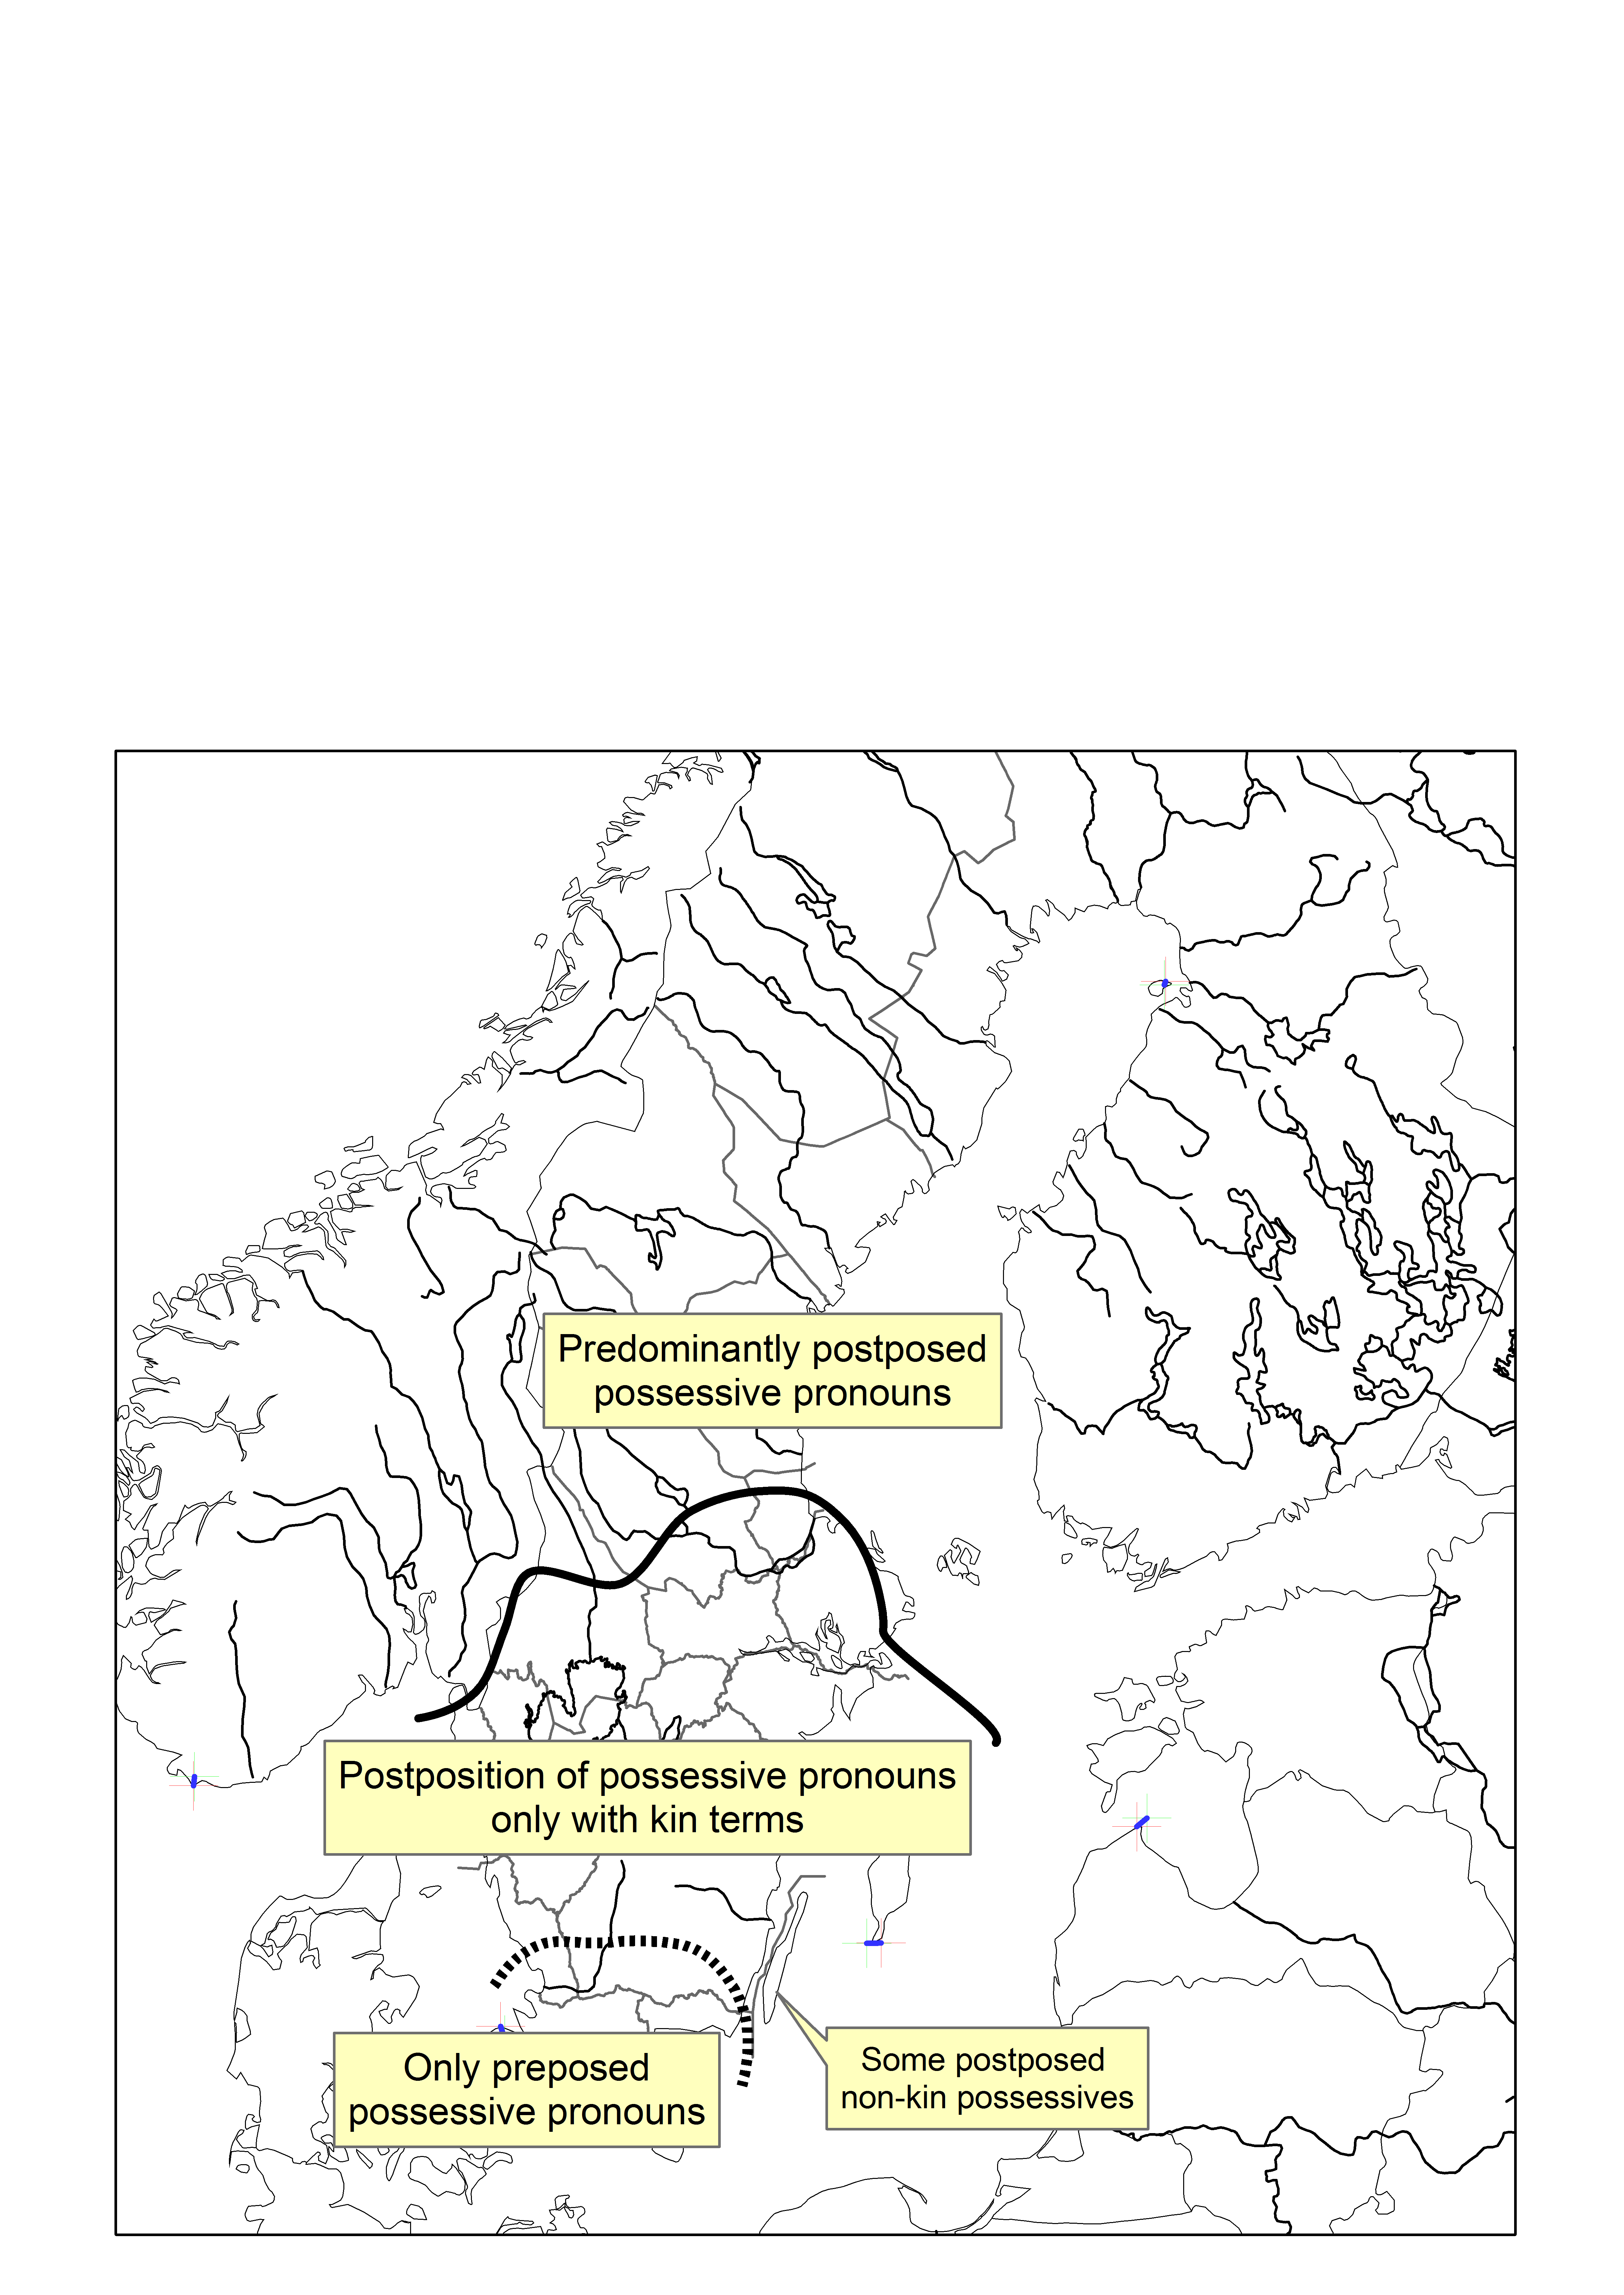
\includegraphics[height=.5\textheight]{figures/25_PlacementofPosPron}
\caption{Placement of possessive pronouns (adapted from \citet{Delsing2003a})}
\label{map:21}

\end{figure}

\section{Concluding discussion: The evolution of possessive constructions in the Peripheral Swedish area}

It is not so easy to sort out the geographical patterns in the diversity of possessive constructions in the Peripheral Swedish area, especially in view of their frequent overlapping. Still, a possible scenario can be sketched.

Two constructions that do not overlap to any great extent but rather are in complementary distribution are the plain dative construction and the prepositional construction with \textstyleLinguisticExample{at}. As we can see from \figref{map:18}, the plain dative construction has a discontinuous distribution, the two parts of which are the two parts of which are on opposite sides of the distribution of the \textit{at} construction. Furthermore, the two constructions appear to have similar origins – from external possessor constructions. A dative external possessor construction is attested from Written Medieval Swedish, whereas an external possessor construction with \textstyleLinguisticExample{at} is found in a large part of the Peripheral Swedish area, notably in the areas where the plain dative construction is still alive. It is thus highly probable that the plain dative construction is the older one and that the \textstyleLinguisticExample{at} construction may have replaced it in Middle Norrland. 

Even if there are some discrepancies (see \sectref{sec:5.5}), the distributions of the \textstyleLinguisticExample{h-}genitive and preproprial articles are similar enough for it to be likely that the former originates in the latter, and Norway is a likely candidate as the origin. Like the plain dative construction, the \textstyleLinguisticExample{h-}genitive has a discontinuous distribution; in fact, the “hole” in the middle is partly the same for the two constructions, and in both cases largely overlaps with the distribution of the \textstyleLinguisticExample{at} construction. Using the same logic as before, we may assume as a possibility that the \textstyleLinguisticExample{at} construction has pushed out not only the dative construction but also the \textstyleLinguisticExample{h-}genitive in parts of Middle Norrland. (Alternatively, the dative was first pushed out by the \textstyleLinguisticExample{h-}genitive, then the \textstyleLinguisticExample{at }construction took over.) Admittedly, we cannot exclude that the coastal \textstyleLinguisticExample{h-}genitive is an independent development. However, one may wonder, if given all the possessive constructions they already had, these vernaculars would have developed another possessive construction if there were no pressure from the outside.

The geographical distribution of the \textstyleLinguisticExample{s}{}-genitive with a definite head suggests that it has expanded from the south along both sides of the Baltic. 

